\chapter[Developed analysis methods for multiple samples and multimodal spatial-omics data]{Developed analysis methods for multiple samples and multimodal spatial-omics data}

\label{Chap:4}	%CREATE YOUR OWN LABEL.
\pagestyle{headings}
\label{Sec:4.1_intro}	%CREATE YOUR OWN LABEL.
\section{Introduction}
The distribution of the cells in a spatial context can determine the crosstalk between different cell types \cite{van2018spatially}. As discussed in chapters \ref{Chap:2} and \ref{Chap:3}, the advances in multiplexing spatial transcriptomic and proteomic (spatial-omics) experimental technologies have enabled us to uncover the complex spatial structure of the tumour microenvironments (TMEs) at an unprecedented resolution and capacity. Using spatial-omics atlas as an approach to recapitulate the intratumoral heterogeneity and the variety of responses across cancer subtypes and/or patients is anticipated to emerge as a routine approach to study cancer tissue \cite{wu2022spatial,napoli2022functional,marsh2022approaches}. A growing number of studies have used spatial-omics technologies to spatially resolve the tumour immune colocalisation within the TMEs, such as breast cancer \cite{jackson2020single, ali2020imaging}, lung cancer \cite{sorin2023single}, colorectal cancer \cite{schurch2020coordinated, pelka2021spatially} and melanoma \cite{nirmal2022spatial}. By combining multiple experimental techniques such as spatial transcriptomic, proteomic and molecular measurements, researchers are aiming to gain a comprehensive view of the cancer status of a biopsy tissue \cite{boehm2022harnessing}. However, barriers around combining different modalities prevent the application of spatial-omics at large quantities \cite{wu2022spatial, vickovic2022sm}. Therefore, methods for computational integration of spatial omics are needed and can provide the key to uncovering the complexity of cell-cell interactions and TMEs from multidimensional data.  
 
Single-cell spatially resolved technologies have allowed us to study the complexity of the TME with unprecedented resolution. Across the TMEs, a number of inter- and intra-tumour heterogeneity is driven by aberrant inter-cellular interactions. Several analysis frameworks for analysing spatial data have been developed (discussed in Chapters \ref{Chap:Intro}). However, there are a limited number of computational frameworks able to perform multiple sample comparisons and multimodal spatial-omics data integration. Although existing software packages offer versatile functions to analyse different spatial-omics data, the implementation is usually applied to individual regions of interest (ROI) and/or the single spatial-omic platform (\ie squidpy\cite{palla2022squidpy}, Giotto\cite{dries2021giotto}, stlearn\cite{pham2020stlearn}, histocat\cite{schapiro2017histocat}). To this aim, we developed an interactive analysis package called Multi-Omics Spatial Analysis Platform (MOSAP), focusing on data combinations from multiple spatial-omics data types and samples and identifying the network heterogeneity across ROIs and/or images. 

MOSAP has been developed to effectively address the challenges associated with the analysis of multiple samples. One of the key features integrated into MOSAP is the scoring of spatial network heterogeneity in cell-cell neighbourhoods and cancer-immune infiltration. We incorporated entropy function\cite{botta2005rao} from the information system field into MOSAP to measure the diversity of cell spatial networks across the ROIs. It is well-known that cell-cell interactions play a critical role in shaping the spatial variability of immune and cancer cells. Numerous cell populations in a TME contribute to the interaction and heterogeneity. Several entropy scores have been widely used to quantify the diversity and complexity of data in the field of information systems or ecology (\ie Shannon entropy, Renyi entropy, Simpson Index or Rao quadratic entropy). In the context of spatial analysis, a similar quantification metric can be applied to study the heterogeneity of the cell neighbourhood network \cite{pienta2008ecological, botta2005rao, martinelli2022athena}. As cell-cell interactions are influenced by both cell types and pairwise distance between cells, we reasoned that the variation of cell spatial organisation also needed to consider the distance between cells. Therefore, Rao quadratic entropy emerged as a suitable metric and was incorporated into MOSAP. The specific implementation of the metric is going to be discussed in Section \ref{Sec:4.2_Methods}. 

Additionally, MOSAP also offers a seamless image registration function to map the spatial coordinates of multiple adjacent tissue sections or tissues with similar structures. This registration process is particularly useful in aligning the spatial coordinates of two tissues, thereby facilitating the integration of multiple spatial omics data. The image registration is available in both graphical user interface (GUI) mode and Python script-based approach. MOSAP provides user-friendly interfaces and powerful analytical features to unravel the spatial dynamics underlying cancer-immune cell interaction across multiple ROIs.

In this Chapter, we demonstrate the robustness of MOSAP in studying cellular colocalisation and cell type heterogeneity using samples from two cancer datasets: skin cancer and colorectal cancer (Table \ref{table:Chapt4_DataInfor}). The first dataset features the spatial transcriptomic using the CosMx platform, which captures a panel of $960$ immuno-oncology genes. Additionally, we extended the analysis of the spatial proteomic data to include Imaging Mass Cytometry (IMC) data for the colorectal cancer samples from Chapter \ref{Chap:3}. Notably, the analyses of this chapter focus on the association of cellular neighbourhoods or TMEs with clinical outcomes and genome alteration like Microsatellite Instability (MSI) (Table \ref{table:Chapt4_IMC_patient_metadata}). 

We further study the cell-cell interaction and colocalisation in the skin cancer samples using the single-cell spatial transcriptomic platform. In this chapter, the transcriptome profile of the cell is captured at higher throughput using a panel of $960$ immuno-oncology genes with the CosMx platform in comparison to a 6-plexed panel RNAscope (Chapter \ref{Chap:2}). Thanks to the increased number of transcripts that can be captured in CosMx data, we can identify cell type and cell-cell interaction through ligand receptors with higher accuracy and confidence \cite{he2022high}. The skin cancer dataset contains $8$ skin cancer samples from patients with SCC, BCC and Melanoma. The fixed tissues were in-situ hybridised with fluorescent probes for the CosMx instrument and scanned using the fields of view (FOVs) approach. Therefore, each skin tissue was scanned into multiple FOVs. By default, each FOV has the dimension of $0.7 \times 0.9 mm^{2}$, which can scan the gene expression of up to $6000$ cells. As the cell segmentation has been done as a standard cycling fluorescent imaging pipeline within the CosMx instrument, the analysis method and discussion in the chapter will focus on the downstream analysis of TMEs heterogeneity and cell colocalisation analysis.

Microsatellite status has been identified as a genetic alteration phenomenon that commonly occurs in colorectal cancer (CRC) \cite{battaglin2018microsatellite}. While MSI-positive is often associated with poor responses to chemotherapies, it has been identified that patients with MSI-high responded better to immunotherapies, particularly in the cases of primary tumour advanced to stage II and stage III CRCs \cite{battaglin2018microsatellite,kawakami2015microsatellite, li2021quantitative}. Therefore, MSI screening has become the recommended test for patients after being diagnosed with CRC and opened a potential field for precision treatment of CRCs \cite{svrcek2019msi}. Common MSI testing involved IHC staining and polymerase chain reaction (PCR)–based methods \cite{umar2004revised}. In order to further explore the spatial association of TMEs with clinical outcomes, we extended the analysis of cell neighbourhoods in the colorectal cancer dataset to investigate the correlation between cell neighbourhoods and MSI status (Table \ref{table:Chapt4_IMC_patient_metadata}). Additionally, the analysis of the IMC dataset also aims to identify the correlation between spatial distribution and survival outcomes in CRC. 
% *********
\begin{table}[ht]
\centering
\caption{Summary of data available}
\begin{tabular}{||P{4cm} || P{5cm} || P{5cm} || } 
 \hline
 Cancer type  & Skin Cancer Samples  & Colorectal Cancer Samples \\ [0.33ex] 
 \hline\hline
 Number of patients & 8 & 52  \\ 
 \hline
 Number of markers & 960 oncology panel CosMx  & 16 proteins panel IMC \\ 
 \hline
 Spatial technology & spatial transcriptomic & spatial proteomic  \\ 
 \hline
 Number of images & 86 FOVs &  172 ROIs \\
 \hline
 Cancer type & BCC/SCC and Melanoma & Stage III colorectal adenocarcinoma \\ [1ex] 
 \hline
 Sample includes  & 2 SCC, 2 BCC and 4 melanoma patients  & 164 tumour and 8 normal ROIs  \\ [1ex] 
 \hline
\end{tabular}
\label{table:Chapt4_DataInfor}
\end{table}
With MOSAP's spatial network analysis, we could identify several significant correlations between the cell-cell neighbourhood and clinical outcomes (or diagnostic, genomic status, survival outcome). Furthermore, the MOSAP platform enables the capture of the spatial neighbourhoods of cells through network modelling. By aggregating similar observations, such as neighbourhood heterogeneity or enrichment scores, we can effectively compare and integrate multiple samples. Overall, we present a computational platform that can quantitatively compare the compositional variation of TMEs across multiple samples and model spatial-omics data. Additionally, the MOSAP package includes user-friendly graphical interfaces and displays of cell segmentation for the CosMx dataset into napari \cite{chiu2022napari} for users without programming backgrounds. 
% *********
\section{MOSAP-MultiOmics Spatial Analysis Platform}
\label{Sec:4.2_Methods}
\subsection{Main components and data structure for multiple samples spatial-omics data}

\begin{figure}
    \centering
    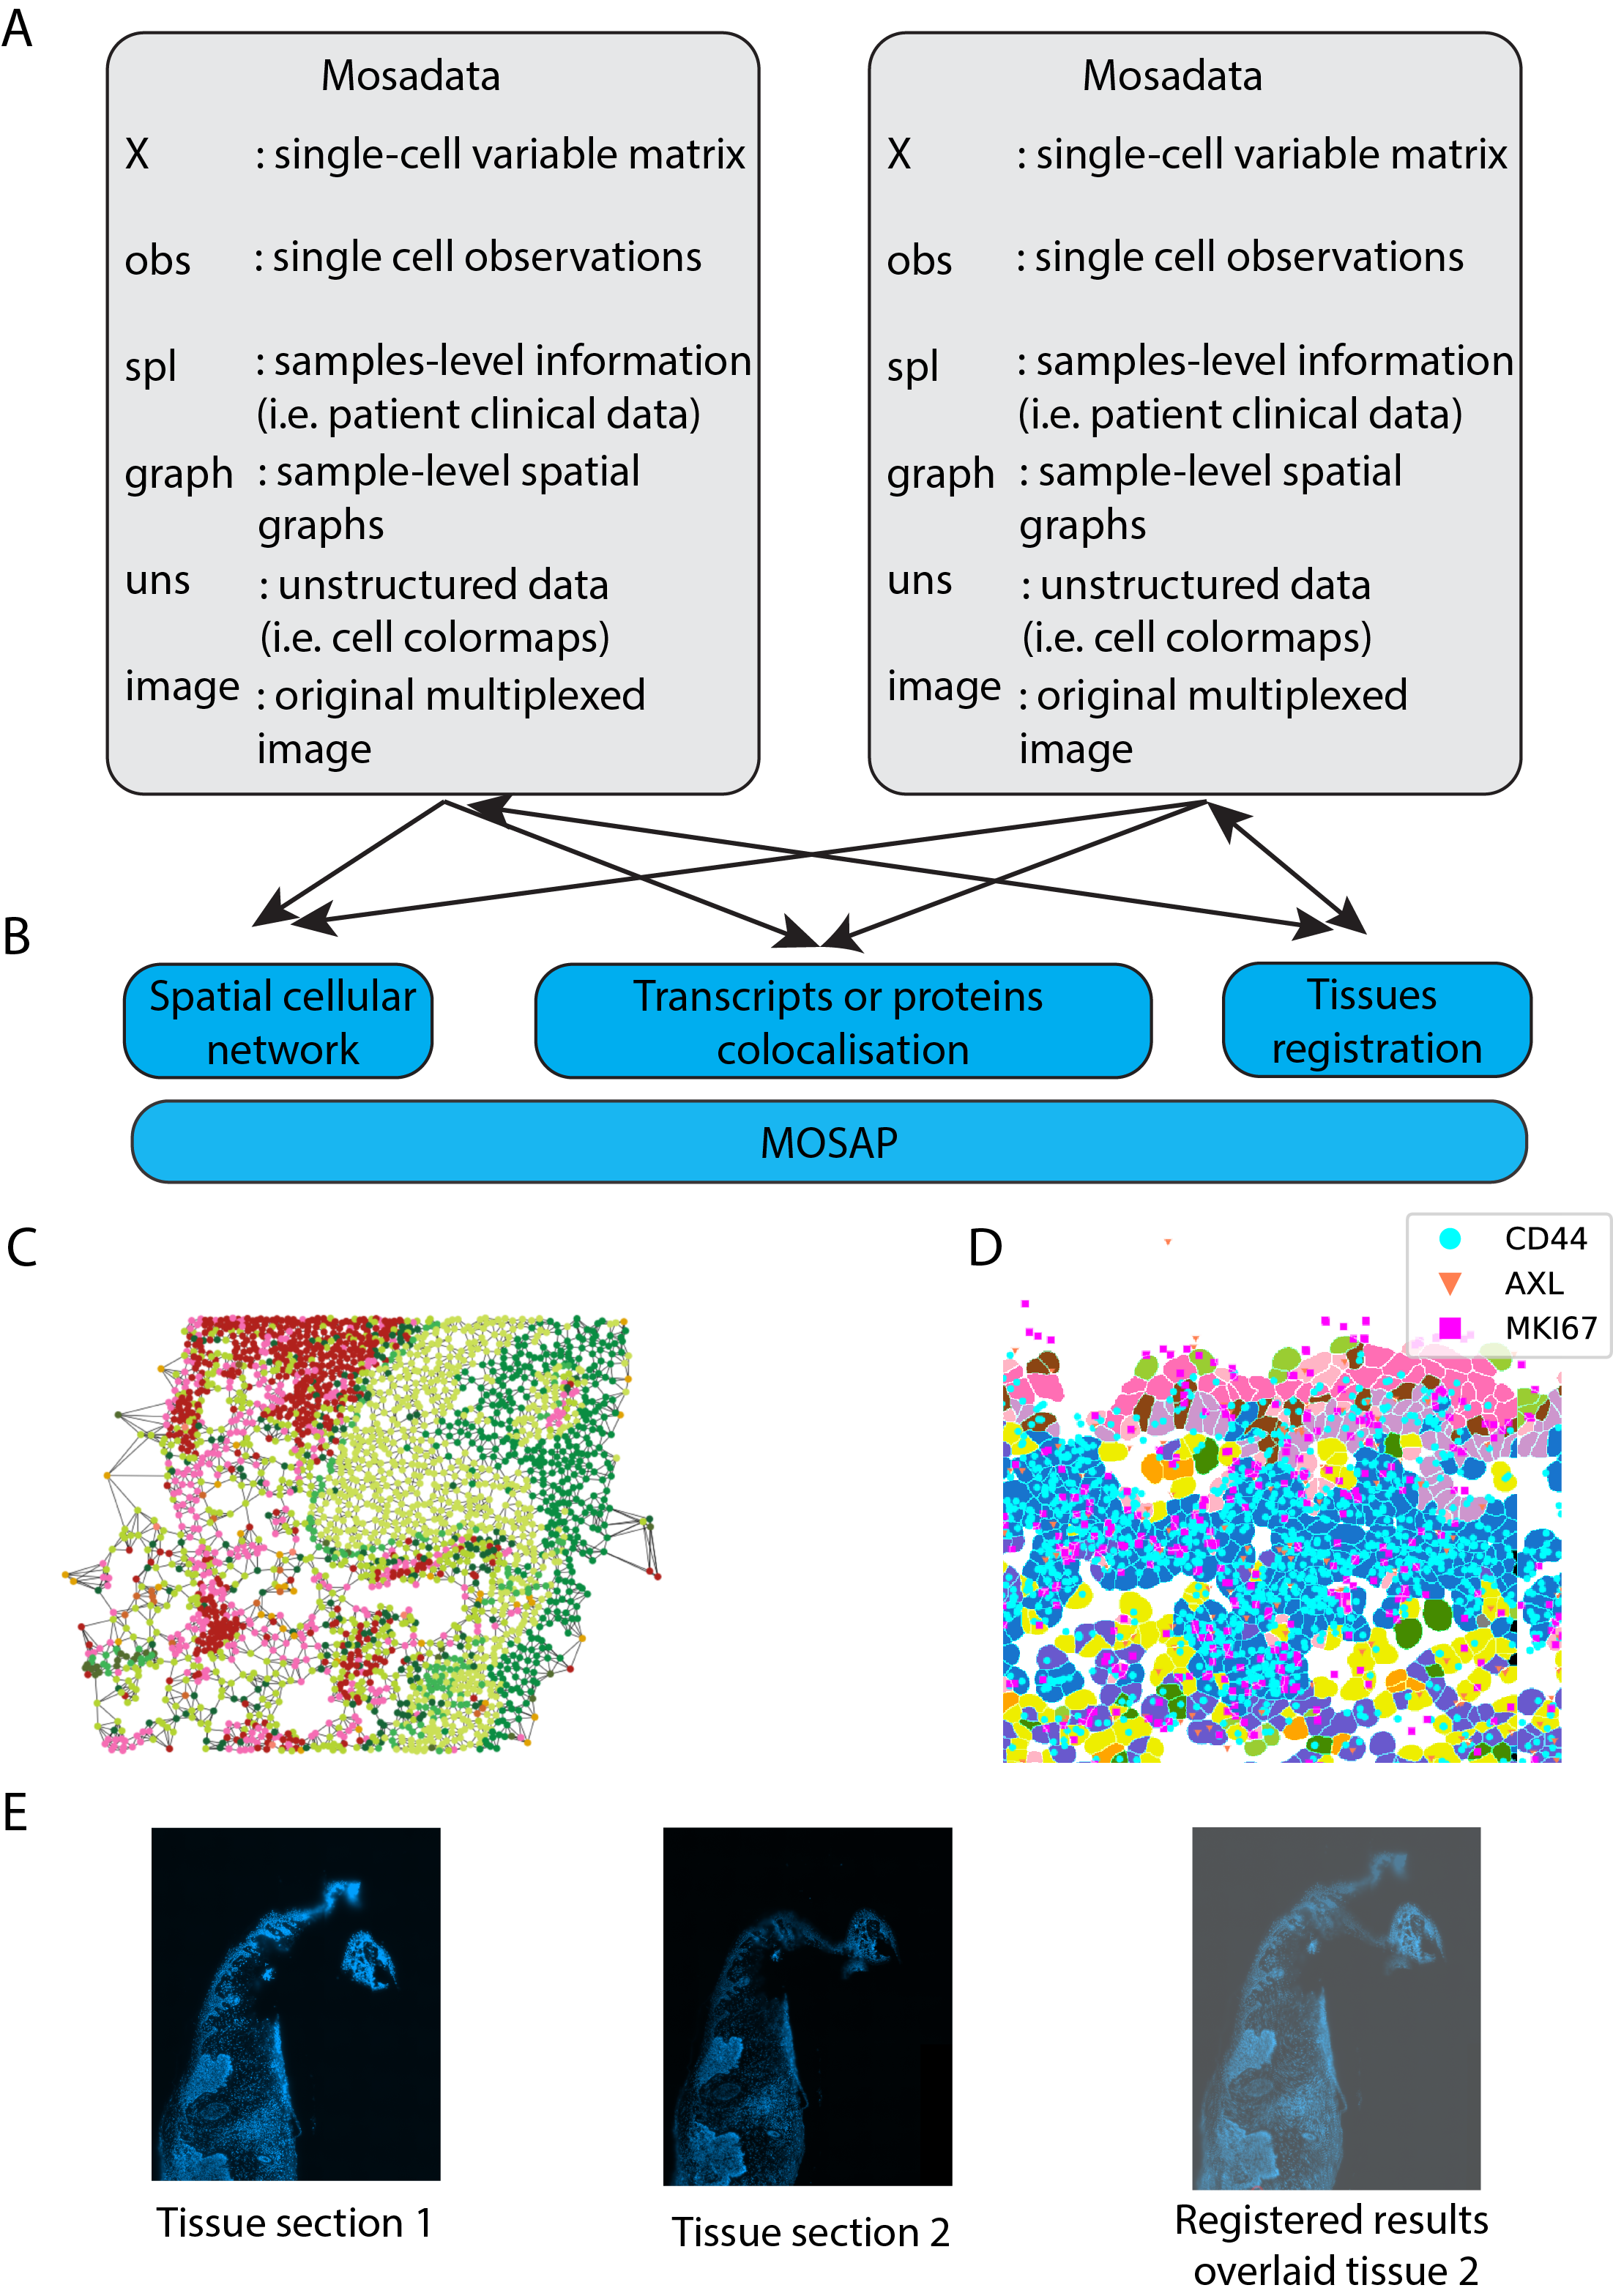
\includegraphics[width=0.8\columnwidth]{Chapter4/Figures/Chap4_MOSAP_DS.png}
    \caption[Schematic illustration of the Mosadata object as the building block of MOSAP]{Schematic illustration of the Mosadata object as the building block of MOSAP. (A) Mosadata is an object designed to store and process spatial-omics data from different experimental designs. (B) MOSAP acts as a platform that enables various spatial analyses, including tissue registration, cell type colocalisation and spatial cellular networks analysis platforms. (C) Multiple network modelling approaches of spatial-omic data are available within MOSAP for sample variational analysis. (D) A feature of MOSAP for identifying the transcripts and proteins co-localisation by cell types. (E) MOSAP also provides multiple methods to register two tissues from adjacent sections or tissues with similar landscapes from separated tissues. The software is available on  \href{Github}{https://github.com/BiomedicalMachineLearning/MOSAP}}
    \label{Chap4:fig:MOSAP_OOP}
\end{figure}

MOSAP, implemented in Python, offers a robust platform for downstream analysis and visualization of diverse spatial-omics data. At its core, MOSAP incorporates the \textit{Mosadata} object, designed to handle single-cell spatial-omics data.  The \textit{Mosadata} object is designed to handle single-cell spatial-omics data and the images associated with each spatial modality. The \textit{Mosadata} contains two key levels of information: the single-cell annotation level and the sample-level information (Fig: \ref{Chap4:fig:MOSAP_OOP}A). 

The single-cell annotation level of \textit{Mosadata} comprises a single-cell expression matrix, denoted as $X$, and an observation attribute matrix, represented as $obs$. The single-cell expression matrix, with the size of the number of cells ($\#cells$) by the number of features ($\#features$), captures the gene or protein expression information for each individual cell. Specifically, $\#cells$ represents the number of cells, and $\#features$ indicates the number of measured biomarkers. Meanwhile, the observation matrix, $obs$, provides additional information to the single-cell expression matrix, including cell type, spatial coordinate, morphological feature, size and shape. 

Building upon the single-cell annotation layer, \textit{Mosadata}'s sample-level layer stores the information about patient clinical relevant data, cell-cell spatial graph ($graph$), supported attributes ($uns$) and the original multiplexed image of the sample ($image$) Fig: \ref{Chap4:fig:MOSAP_OOP}A). Importantly, each instance of \textit{Mosadata} provides an option to store the original multiplexed image of a sample, facilitating the interactive feature of the single-cell annotated data. The object is compatible with spatial data at multiple levels, from transcript/protein to cellular and sample levels. Furthermore, the \textit{Mosadata} object seamlessly integrates with existing data structures such as \textit{AnnData} from scanpy \cite{wolf2018scanpy} and \textit{SpatialOmics} from ATHENA \cite{martinelli2022athena}, enhancing compatibility and supporting a wide range of analysis pipelines.  

Although the design of \textit{Mosadata} is inspired by \textit{AnnData} architecture \cite{wolf2018scanpy}, there are two critical differences in separating two data objects. Firstly, \textit{Mosadata} object is implemented using a sample-centric approach, where data matrices and observations for each sample are stored separately. As the throughput or list of observing markers of each sample varies, resulting in non-overlapping gene and/or protein panels across samples. However, the single cell expression matrix instance ($X$) from \textit{AnnData} requires two datasets to have identical lists of $\#features$ to be merged. Secondly, MOSAP enables flexible visual inspection of results by treating each sample as an individual instance. By storing each sample individually, \textit{Mosadata} allows data exploration of each sample, facilitating detailed analysis within the context of the specific sample. With the new design for the data structure, MOSAP allows the analysis across samples and incorporates multiple spatial-omic data together without concern about the dissimilarity between modalities.

We developed MOSAP with three key features that are tightly interwoven with \textit{Mosadata} (Fig: \ref{Chap4:fig:MOSAP_OOP}B). Firstly, MOSAP is implemented with a function for multiple tissue registration, which allows aligning tissues with similar morphology and/or anatomical structures (Fig: \ref{Chap4:fig:MOSAP_OOP}C). Unifying the coordinate planes of two or more tissue samples can allow us to integrate data generated by multimodal experiments. This feature is particularly valuable in the context of spatial multi-omics analysis.

Secondly, we introduced cell-type neighbourhood enrichment analysis through transcripts colocalisation. As the throughput of the spatial data increases, certain cell types may exhibit spatial proximity and demonstrate enrichment in transcripts or protein colocalisation (Fig: \ref{Chap4:fig:MOSAP_OOP}D). This feature possibly allows for a deeper understanding of the spatial relationships between cell types through ligand-receptor (L-R) pairs.

Finally, MOSAP can construct four different types of cellular networks given an input sample (Fig: \ref{Chap4:fig:MOSAP_OOP}E). These networks can capture various aspects of cellular interactions through space within the tissue. In the subsequent sections, we will detail the usage of each feature, showcasing their utilities to capture the variation of cell heterogeneity and model the neighbourhood relationship between cell types. Further details about each of the MOSAP cell-cell neighbourhood analysis features will be discussed in the following sections. 

\subsection{Constructing cell-cell neighbourhood networks}
A cellular neighbourhood network is a network representation of tissue where each cell is a node and neighbourhood relations between cells are edges. Through the analysis of these cell neighbourhood networks, we can understand the global co-expression patterns and capture higher-order relationships among different cell types across samples or ROIs. MOSAP constructs the spatial graphs stored in the networks in the \textit{Mosadata}'s $graph$ attribute using the Python dependency called networkx \cite{hagberg2008exploring}. The $graph$ attribute retains the pairwise distance between neighbouring cells within the network, enabling the calculation of various network measurements such as node entropy and graph connectivity. We implemented three kinds of networks to model different types of cell-cell neighbourhoods and interactions. The detailed implementation and usage cases of each network model will be discussed in the following sessions. To demonstrate the MOSAP's ability to measure the spatial variation across samples, we performed spatial cell type colocalisation and heterogeneity measurement across samples using network analysis. The results of this analysis demonstrate how effective MOSAP can be in deriving high-level interpretation of spatial relationships. 

In the MOSAP heterogeneity feature, we implement Rao’s quadratic entropy \cite{pienta2008ecological,botta2005rao} function to measure the diversity of connection between the observing cell and neighbouring cells (\ie two cells sharing an edge). Utilising Rao’s quadratic entropy scoring as a measurement for heterogeneity has two advantages. Firstly, the entropy score considers the probability of two neighbouring cells (i.e. two cells sharing an edge) being different cell types, which captures the variability of the neighbouring cells. Secondly, Rao’s quadratic entropy also considers the spatial distance between each node of the neighbouring pair, which is essential for cell-cell interaction through paracrine signalling. To quantify the heterogeneity of a cell neighbourhood network, Rao's quadratic score is formulated by multiplying the joint probability and the pairwise distance between two cells sharing an edge in the network (Equation \ref{chap4:eq:02}). Next, the final score is summing over all the distance, considering the differences in distance between cells $d(x_i, x_j)$, as well as the frequencies $p(x_i)$ and $p(x_j)$ of the two neighbouring cells belonging to different cell types.      

\begin{equation}
    Rao\_score = \sum^{S-1}_{i=1}\sum^{S}_{j=i+1}d(x_i, x_j)p(x_i)p(x_j)
\label{chap4:eq:02}
\end{equation}

We conducted spatial heterogeneity analysis on both the skin cancer and colorectal cancer datasets using MOSAP. For each input image, the Rao quadratic score was applied to the annotated cells to measure the overall heterogeneity of each neighbourhood network. The scores from multiple ROIs were aggregated by samples using sample-level information from \textit{Mosadata}. The heterogeneity measurement relies on the choice of neighbourhood network and is unaffected by the total number of cells per ROI or FOV. Therefore, the choice of neighbourhood network is essential for comparing the heterogeneity score across samples. In the skin cancer dataset, the spatial analysis allowed us to assess the variation in cell-cell neighbourhood networks across different FOVs and highlighted the differences in the heterogeneity between BCC, SCC and Melanoma. Similarly, we could also identify the correlation between cell neighbourhoods and MSI status, as well as the survival outcomes, by extending the investigation of cell neighbourhoods in the colorectal dataset.          

\subsubsection{Radius network}
MOSAP provides a function to construct cellular networking by scanning for the presence of cells within a radius apart from each cell in the spatial-omic data (Fig \ref{fig:Chap4_networks_models}A). By utilising the radius network, we can examine the spatial relationships between different cells and simulate paracrine signalling, which involves cell-cell interactions occurring within relatively short distances. For example, we can use the radius network to examine the relationship between cancer cells and immune cells within a certain range and evaluate the extent of their colocalisation and interaction. MOSAP provides a function for the user to query the neighbouring information of every cell within a customisable threshold. The functionality is inspired by the co-occurrence analysis presented in Chapter \ref{Chap:3}. One practical application using this type of network is the calculation of the co-occurrence score, which has proven effective in capturing significant cellular interactions, including ligand-receptor pairs. By leveraging the radius network, MOSAP facilitates a deeper understanding of the cellular interaction, including ligand-receptor pairs and cell-type neighbourhood enrichment underlying diverse cancer development processes.        

\subsubsection{K nearest neighbour network}
In addition to the radius network, MOSAP also has the ability to build the cellular neighbourhood network using the K nearest neighbour (KNN) approach. The KNN network is achieved by scanning the K nearest cells surrounding the observing cell in the spatial-omic data and connecting them to the same network. Unlike the radius network, KNN is not restricted by the fixed distances threshold, which means the pairwise distance between two neighbouring cells in the network can vary. While KNN is also suitable for modelling cell-cell interactions through paracrine signalling, this type of network is affected heavily by the densities of the cells per sample (Fig \ref{fig:Chap4_networks_models}B). Therefore, distance cut-off and/or normalisation would be required for this network model to compare across samples. To address this, we have implemented a distance cutoff function that can be used for post-processing the cellular network within MOSAP to enable sample aggregation. By retaining the pairwise distance of nodes in the network, the KNN network can facilitate the study of cell-cell colocalisation through paracrine signalling and the analysis of the neighbourhood relationship between cells.

\subsubsection{Delaunay neighbourhood network}
In addition to the KNN and radius networks, MOSAP also offers the option to construct a Delaunay network, which is a parameter-free approach for capturing cell-cell neighbourhoods. Specifically, a Delaunay triangle is formed by connecting the circumcircles of any group of three points \cite{fortune1995voronoi}. In the context of spatial-omic, a group of three discrete cells are connected in a graph if each cell is an angle in the Delaunay triangle. Unlike the KNN approach or radius network, which relies on a pre-defined number of neighbouring cells and the radius network that depends on the distance threshold, the Delaunay network connects cells based on their spatial relationships. This type of network is not only parameter-free but also robust enough to avoid the problem with the interaction of the set of cells on the same straight line (Fig \ref{fig:Chap4_networks_models}B-C). By utilising the Delaunay network or other type of neighbourhood network method, MOSAP can provide an additional method to capture cell-cell neighbourhoods and facilitate the calculation of various network metrics (\ie heterogeneity and connectivity) for downstream analysis.   

\begin{figure}[htp]
    \centering
    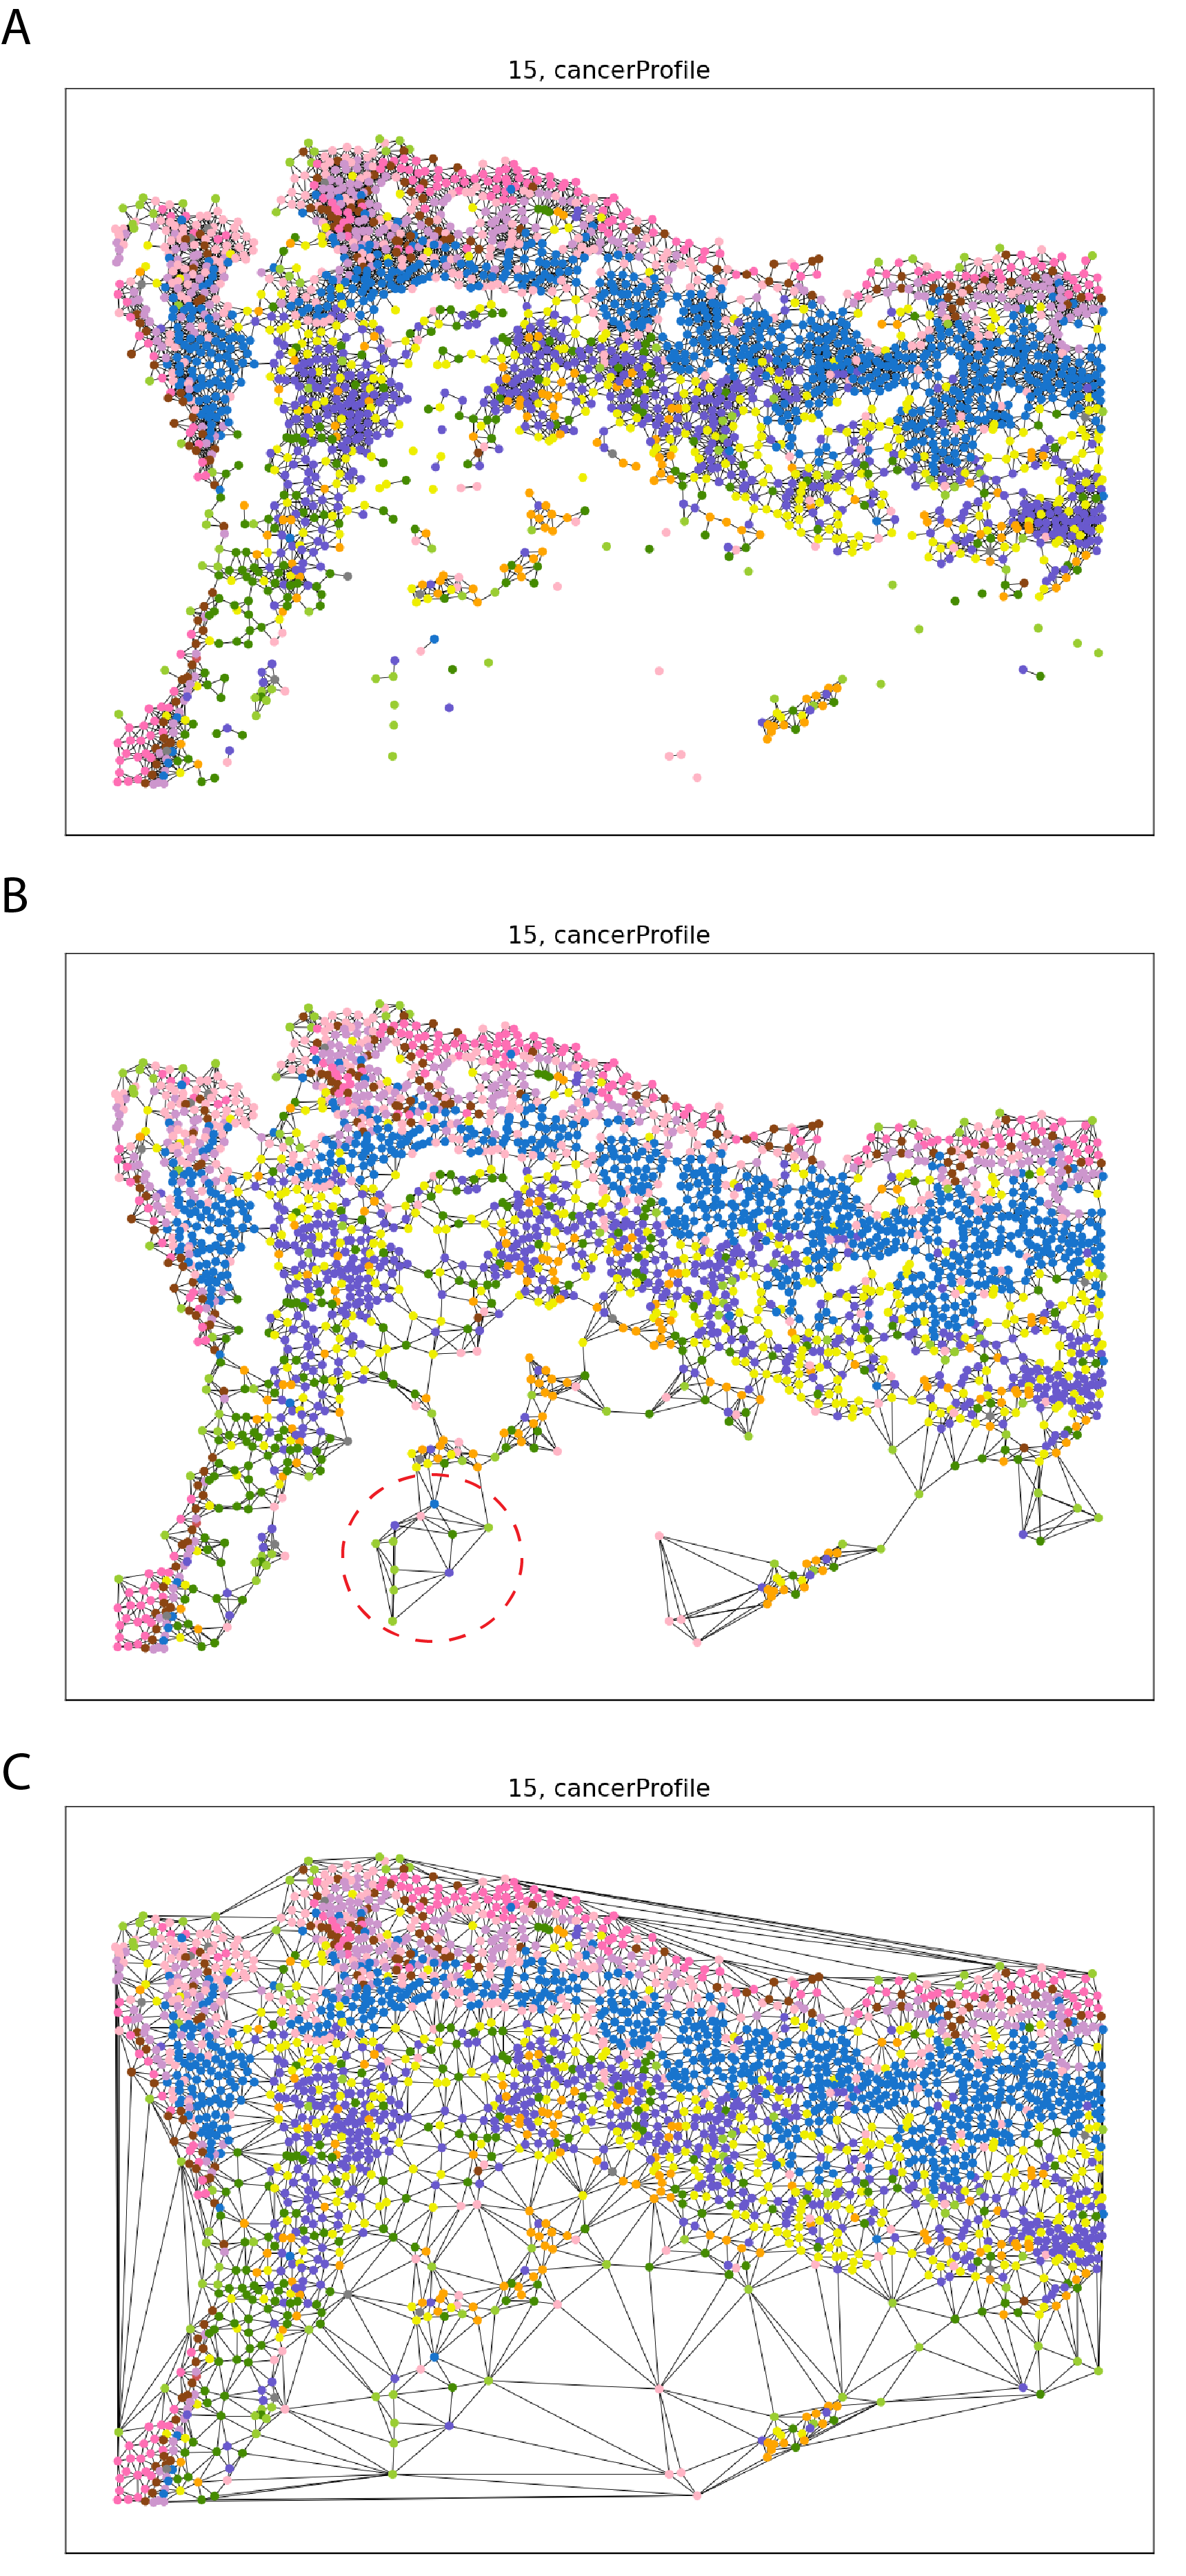
\includegraphics[width=0.6\columnwidth]{Chapter4/Figures/Chap4_neighbourhood_networks_appendix.png}
    \caption[Examples MOSAP networks in CosMX data (FOV15)]{Example of MOSAP networks in CosMX data (FOV15).(A) An example of radius neighbourhood network. (Legend continues on the following page.)}
    \label{fig:Chap4_networks_models}
\end{figure}
\begin{figure}[t]
  \contcaption{(B) The K nearest neighbour (K=6) networks modelling of cells in FOV15. The red circle highlighted the incident when 4 cells in a line are connected in the neighbourhood network. (C) Delaunay network modelling of the same FOV.}% Continued caption
\end{figure}
\subsection{Quantifying spatial enrichment of cell type colocalisation}
In addition to spatial heterogeneity, the cellular neighbourhood network can also facilitate the spatial enrichment analysis. In this approach, the total count of interaction of a cell is represented by the number of edges that originate from that cell. The spatial enrichment analysis quantifies the frequency of pairwise interaction between cell types and compares the actual interaction score (baseline interaction) with a randomised permutation of cell types. The permutation test is conducted by shuffling cell labels(nodes) in the cell spatial network while retaining the neighbourhood connection(edges). Next, the average neighbourhood score is recomputed for the observed interaction for every iteration of the random shuffling. The obtained distribution of baseline and observed interaction allows us to compute $p-value$ and $z_score$ for the neighbourhood interaction of cell types. Unlike the permutation test in squidpy \cite{palla2022squidpy}, our implementation also considers the source and target cells of an interaction, which provides more granularity into how cells interact with each other.n Throughout the permutation test, the total interaction counts of each cell type are used as the normalisation factor enrichment score.    

More specifically, two variables were defined, $source_celltype$ and $target_celltype$, to form the count matrix of neighbourhood interaction (also known as neighbourhood enrichment). Firstly, the function counts the total number of edges started from each $source_celltype$ node in the neighbour networks and groups edge count by $target_celltype$. Secondly, the raw count of the pair $source_celltype$-$target_celltype$ will be normalised by the total number of edges started from $source_celltype$ to compute the baseline neighbourhood score. Next, the random permutation of cell type is applied to shuffle the label of cells while keeping the connectivities. The neighbourhood score is recomputed for each iteration of permutation. The differences between baseline and randomised neighbourhoods (Equation \ref{chap4:eq:03} )allow us to determine whether the interaction between any pair of $source_celltype$-$target_celltype$ was enriched for interaction or avoidance. Furthermore, the neighbourhood enrichment scores across multiple FOVs and ROIs can be aggregated for comparison across multiple samples. The enrichment score was leveraged from the permutation approach from histocat (\cite{schapiro2017histocat}) and squidpy(\cite{palla2022squidpy}).

\begin{equation}
    zscore_{source_celltype, target_celltype} = \frac{baseline - observed\_mean{(source_celltype, target_celltype)}}{std_{(baseline, observed)}}
\label{chap4:eq:03}
\end{equation}
\subsection{Seamlessly registration of images from adjacent tissue sections}
After performing imaging for techniques such as fluorescence in situ hybridization (FISH) or multiplexed immunofluorescence (IF), the fluorescence probes are usually hybridised by heat treatment for sequential staining. However, this imaging process can easily damage or ablate the tissues, making it challenging to retrieve RNA/DNA and protein from the same section \cite{chen2015spatially, wang2012rnascope, hoyt2021multiplex}. To overcome this challenge, multimodal experimental designs are often performed on adjacent tissue sections. Consequently, the current imaging routine often involves using multiple adjacent tissue sections, with each section as the sample for a single spatial-omic dataset. A registration function can act as an intermediate stage to combine tissue samples from multiple spatial-omic platforms. Additionally, the registration can also enable the alignment of multiple tissue samples with similar morphology from different tissue blocks. The images can be registered together using the $tissue\_registration$ function or $MultiOmic registration$ widget from MOSAP. 

MOSAP offers five different image transformation methods to facilitate the registration process. Here, we define two variables $moving\_img$ and $ref\_img$ representing the registering and reference input images for the registration function, respectively. The first three methods enable basic image transformation for image rotation, translation and bilinear interpolation. More specifically, image rotation and image translation allow shifting the hyperplane of the $moving\_img$ to a new degree or a new position along the $ref\_img$'s xy-axis. Meanwhile, bilinear interpolation can scale up the $moving\_img$ to match the size of $ref\_img$ by estimating the pixel values of the surrounding known pixels. These three registration methods have been widely used for multi-resolution registration of MRI and CT scan images \cite{leng2013medical}. These methods are particularly useful for aligning the coordinate planes and macro-displacement of the input images. However, these basic image transformations may not address the structural misalignments that accumulate due to micro-variations in imaging processes.

In addition to the rotation and translation, MOSAP offers more advanced techniques to facilitate image registration. One of these methods is the Affine transform, which can shear and scale the image $moving\_img$. More specifically, the Affine transform can anchor the changes to some specific sub-regions of the $moving\_img$, which is particularly useful for aligning local regions in preparation for global transformation (Fig: \ref{Chap4:MOSAP_registration}A). MOSAP also provides a B-spline transform to support higher-order of registration. The B-spline transformer maps the global structures of the $moving\_img$ to the $ref\_img$ using B-spline curves. The curves are determined by connecting a sparse set of control points, which are uniformly distributed throughout the fixed $ref\_img$ \cite{shackelford2011deformable} (Fig: \ref{Chap4:MOSAP_registration}A). 

MOSAP uses mutual information scores as the metric to assess the accuracy of the image registration process. Given the images are correctly registered, the joint histogram of the two images should show similar clusters for aligned local and global structures. Therefore, the mutual information score measures the joint probability of co-occurrence of $x$ and $y$ (denoted as $p(x,y)$) being the pixels from two input images, respectively (Equation \ref{chap4:eq:01}). Additionally, MOSAP employs an iterative approach to perform image registration by applying the selected method to transform the grayscale image, $moving_img$, at multiple resolutions to align it with the reference image, $ref_img$. The function aims to maximise the mutual information score between the two images, as defined in Equation \ref{chap4:eq:01}. By iterating through multiple resolutions, MOSAP can achieve the optimal alignment of the two images given a registration function.

\begin{equation}
    mutual\_score_{(moving\_img, ref\_img)} = \sum_{x \in moving\_img} \sum_{y \in ref\_img} p(x,y)log(\frac{p(x,y)}{p(x)p(y)})
\label{chap4:eq:01}
\end{equation}
The mutual information score $mutual\_score_{(moving\_img, ref\_img)}$ is defined by Equation \ref{chap4:eq:01}. The score  $p(x,y)$ is the joint probability distribution of the two images, and $p(x)$ and $p(y)$ are the marginal probability distributions of $moving\_img$ and $ref\_img$, respectively. $mutual\_score_{(moving\_img, ref\_img)}$ represents the amount of information obtained about $moving\_img$ when the value of $ref\_img$ is known, and vice versa.  

\begin{figure}
    \centering
    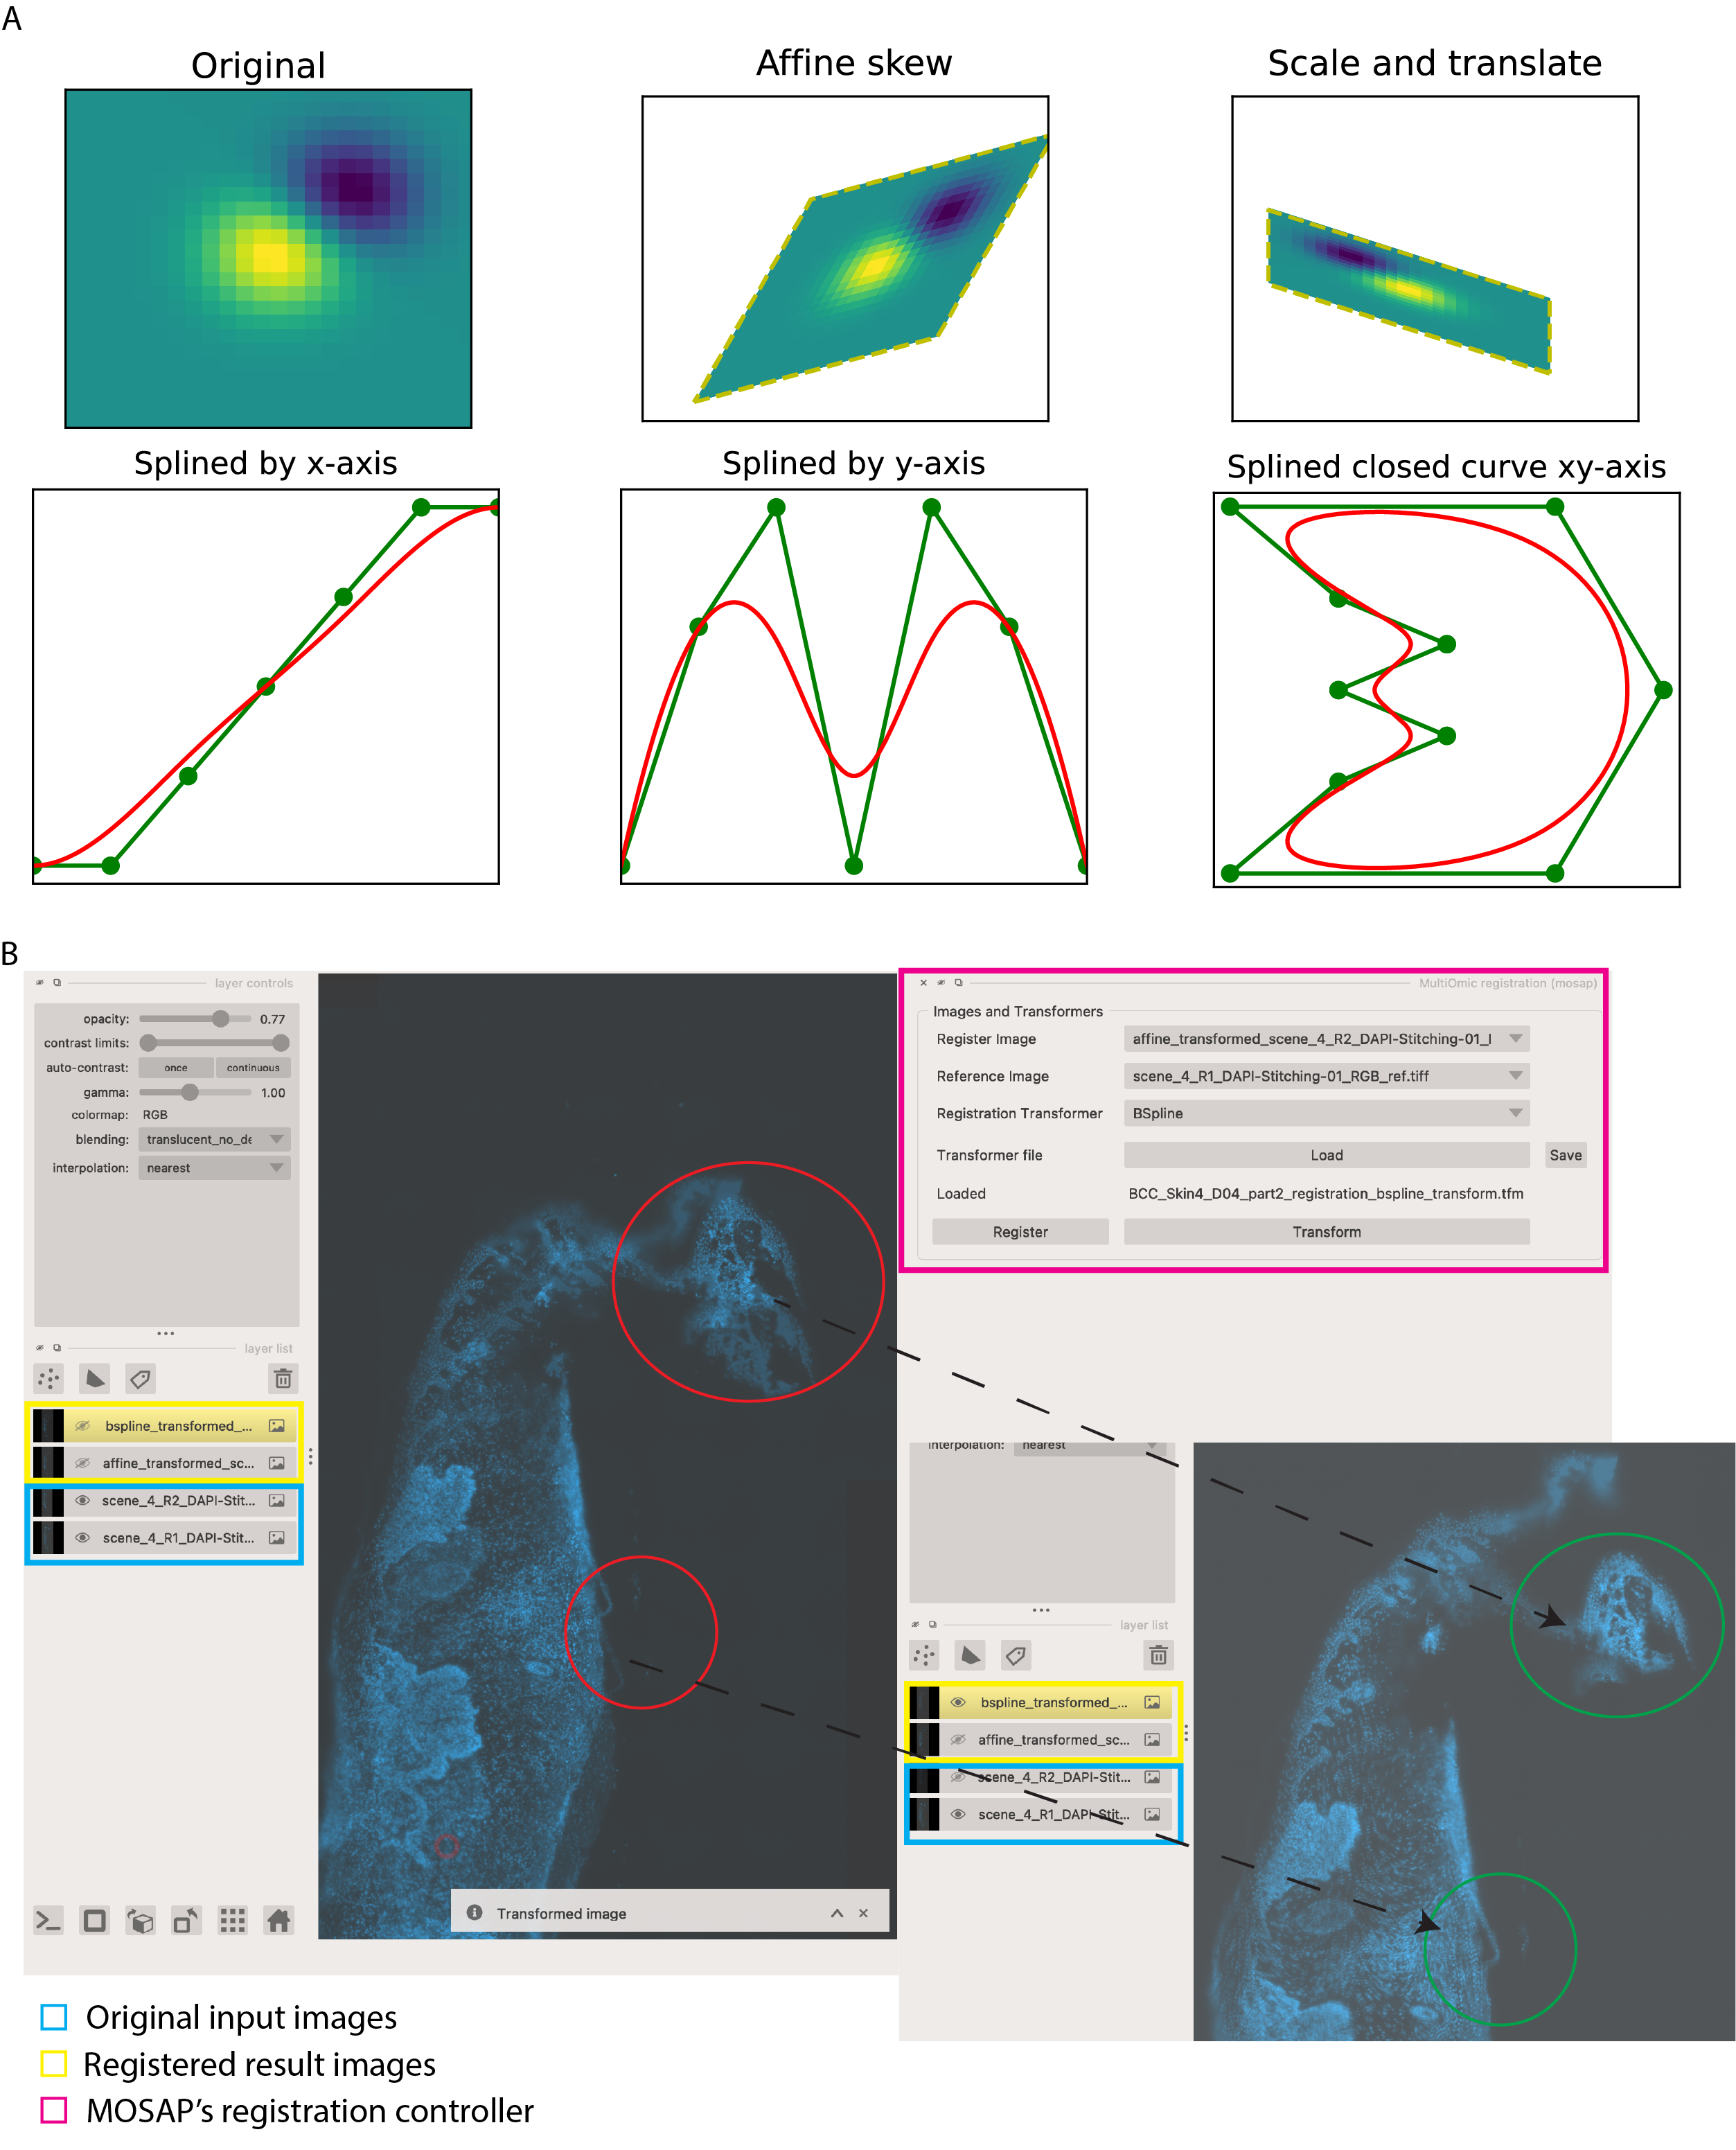
\includegraphics[width=\columnwidth]{Chapter4/Figures/Chapt4_Figure1_registration.png}
    \caption[Graphical interface of MOSAP's registration module]{Graphical interface of MOSAP's registration module. (A) MOSAP provides registration methods to align images of adjacent tissue sections. Using the MOSAP napari plugin, the users can perform the registration seamlessly with multiple transformer options (\ie Affine and B-splines transform*). (B) The visual inspection of the registered image over the reference image can provide an interactive quality check of the registration result. (* Simulation example using scipy Affine transform \cite{SciPy2020NMeth})}
    \label{Chap4:MOSAP_registration}
\end{figure}

\section{Results}
\subsection{Application of MOSAP in differentiating tumour heterogeneity in skin cancer}
As mentioned, CosMx is a platform for spatial transcriptomics at single-cell resolution. With the current number of transcripts in the panel at $960$ genes, CosMx technology is among the highest throughput FISH platform. Given the compelling throughput and resolution, we generated CosMx data for nine skin cancer samples, including three SCC, two BCC and four melanoma samples. Each tissue biopsy was selected for multiple fields of view (FOVs) and underwent the CosMx probes hybridisation. For the computational analysis of the skin cancer dataset, images generated by the CosMx platform were preprocessed single-cell spatial using the pre-trained segmentation model \cite{stringer2021cellpose}. The preprocessing pipeline takes tissue images stained with both nuclear and membrane markers to perform rescaling, normalisation, and boundary enhancement. The preprocessed images were fed into pre-trained Cellpose \cite{stringer2021cellpose} to extract cell boundaries. After cell segmentation, we identified a total of $127,056$ individual cells from $86$ FOVs. Next, we performed cell type identification using the gene expression profile. We clustered and annotated the cell type in the CosMx data into $11$ cell populations (Figure \ref{Chap4:fig1}A). Among the $11$ cell type populations, there were three immune cell clusters, four Keratinocyte (KC) clusters, and tissue-structural specific cell types such as endothelial cells, fibroblasts, melanocytes and pilosebaceous cells. Particularly, $4$ skin-associated Keratinocyte cells were identified namely Basal Keratinocyte(KC-Basal), Keratinocyte-Cycling (KC-Cyc), Differentiating Keratinocyte and other Keratinocyte subpopulations (Figure \ref{Chap4:fig1}A). 

\begin{figure}
    \centering
    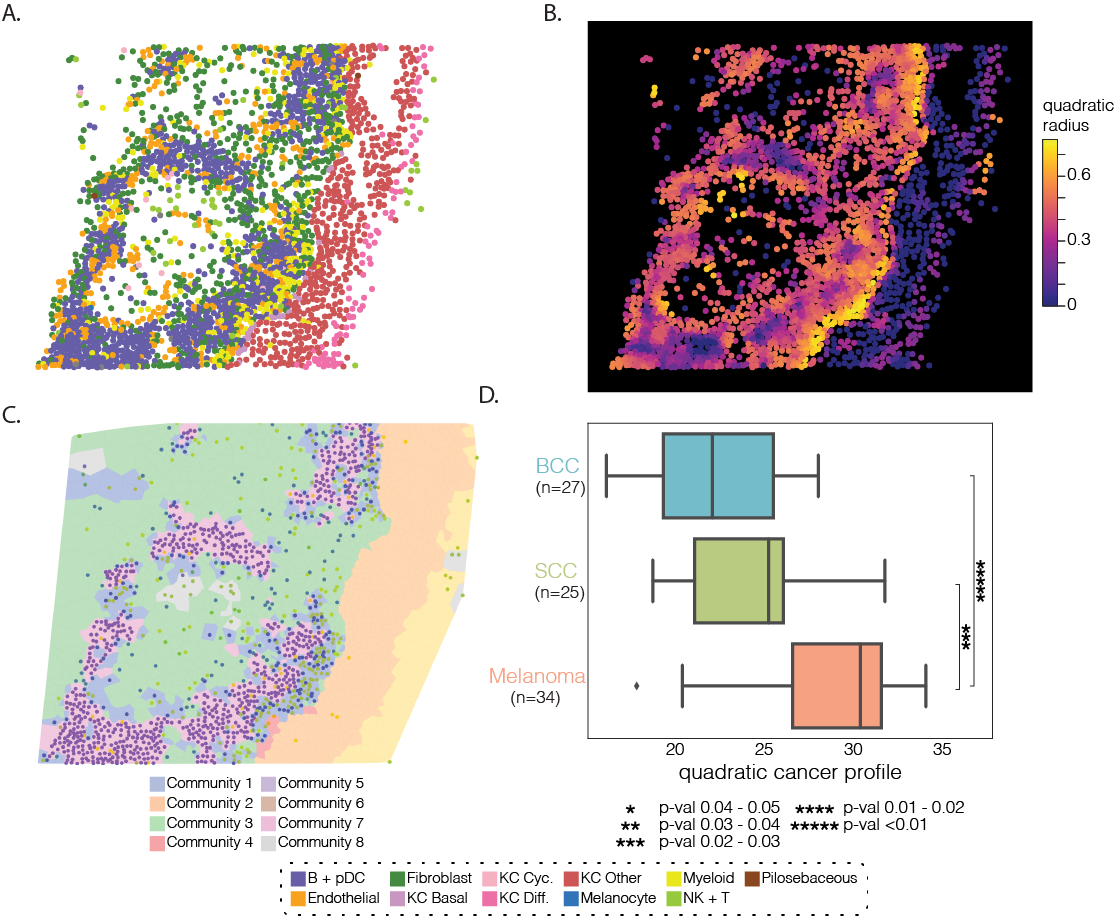
\includegraphics[width=0.8\columnwidth]{Chapter4/Figures/Chap4_figure_2.png}
    \caption[The spatial heterogeneity analysis using CosMx data across the skin cancer subtype]{The spatial heterogeneity analysis using CosMx data across the skin cancer subtype. (A, B) The cell type annotation using CosMx data of patient B18 and the heatmap of the spatial cell heterogeneity from the same FOV. (C) Voronoi diagram of eight cell communities identified in the tissue shown in (A-B) and cell types overlaying of community 7 (pink). (D) Boxplot of heterogeneity scores across three skin cancer types, indicating the most significant overall heterogeneity score for melanoma. The P-value was based on the Wilcoxon rank sum test. }
    \label{Chap4:fig1}
    
\end{figure}

\subsubsection{Generation and quantification of cell neighbourhood network with MOSAP}
To better quantify the complexity and cell type heterogeneity of cell distribution across the dataset, we performed the spatial analysis of cell neighbourhood. The annotated cells were projected back into the original FOVs using their coordination to perform heterogeneity analysis and community detection. Firstly, we used the cell's coordinates to construct the Delaunay neighbourhood network for each FOV. The Rao quadratic score was used to measure the diversity of the cell-cell connections for the cell neighbourhood network of each individual FOV.  This heterogeneity score for each cell was visualised as a heatmap (Figure \ref{Chap4:fig1}B). Given the FOV $15$ from an SCC tissue sample showed the highest overall entropy score, we selected that FOV to explore further the factors contributing to the overall heterogeneity. Next, we performed cell community detection on FOV $15$ to identify the cell neighbourhood that is enriched for the high heterogeneity. By clustering the cell neighbourhood features, we determined $8$ communities of cells from the FOV (Method: \ref{Chap:3:Community_detection_Method}). Qualitatively, the regions within FOV $15$ that exhibited a high level of heterogeneity were enriched for immune cell types, including B cells, plasmacytoid dendritic cells (pDCs), and myeloid and T cells beneath the dermis layer of the skin(Figure \ref{Chap4:fig1}B-C). Voronoi diagram mapping of cell communities also confirmed these spatial regions composed of different groups of cell types. Particularly, community $7$ showed a high density of immune cells (i.e. pDCs and myeloid) consistent with our heterogeneity heatmap (Figure \ref{Chap4:fig1}B, C). Overall, the spatial analysis of cell neighbourhood network and community detection revealed consistent patterns of cell type heterogeneity within the skin cancer dataset, particularly the spatial distribution of immune-dense regions.

\subsubsection{Comparison of TME heterogeneity across skin cancer subtypes}
After performing the spatial heterogeneity across each individual sample, we further measured the overall heterogeneity across all $86$ FOVs to compare cell type heterogeneity across the different cancer subtypes. The heterogeneity scores of each FOV were aggregated and grouped by cancer type to test for heterogeneity variation (Fig \ref{Chap4:fig1}D). The distribution of heterogeneity scores for each skin cancer subtype was pairwise compared using the Wilcoxon test. We observed a significant increase in cell heterogeneity score in the melanoma samples compared to non-melanoma skin cancers, including BCC and SCC (Figure \ref{Chap4:fig1}D). This finding suggests that the cellular microenvironment in melanoma skin contains a wider variety of cell types coexisting than in other skin cancers. 

The sub-cellular capture resolution of CosMx technology also allowed the cellular location of individual RNA molecules to be visualised. We observed the high density of melanoma-associated gene markers, including KMI67, CD44, and AXL, that appeared within the cell areas of Melanocytes (Figure \ref{Chap4:CosMX_transcript_colo}A-C). The neighbourhood interaction analysis also revealed the strong co-enrichment of Melanocytes within the same FOV. The neighbourhood enrichment of Melanocytes with itself is due to the increased proliferation of Melanocytes in melanoma, which is consistent with previous studies (\cite{wang2016crosstalk, shain2016melanocytes}). Additionally, we identified the positive interaction between groups of Keratinocytes, including KC Basal, KC Diff and KC Other. Overall, the spatial heterogeneity and neighbourhood enrichment analysis yield interpretable results when the MOSAP is applied to our skin cancer dataset. 

\begin{figure}
    \centering
    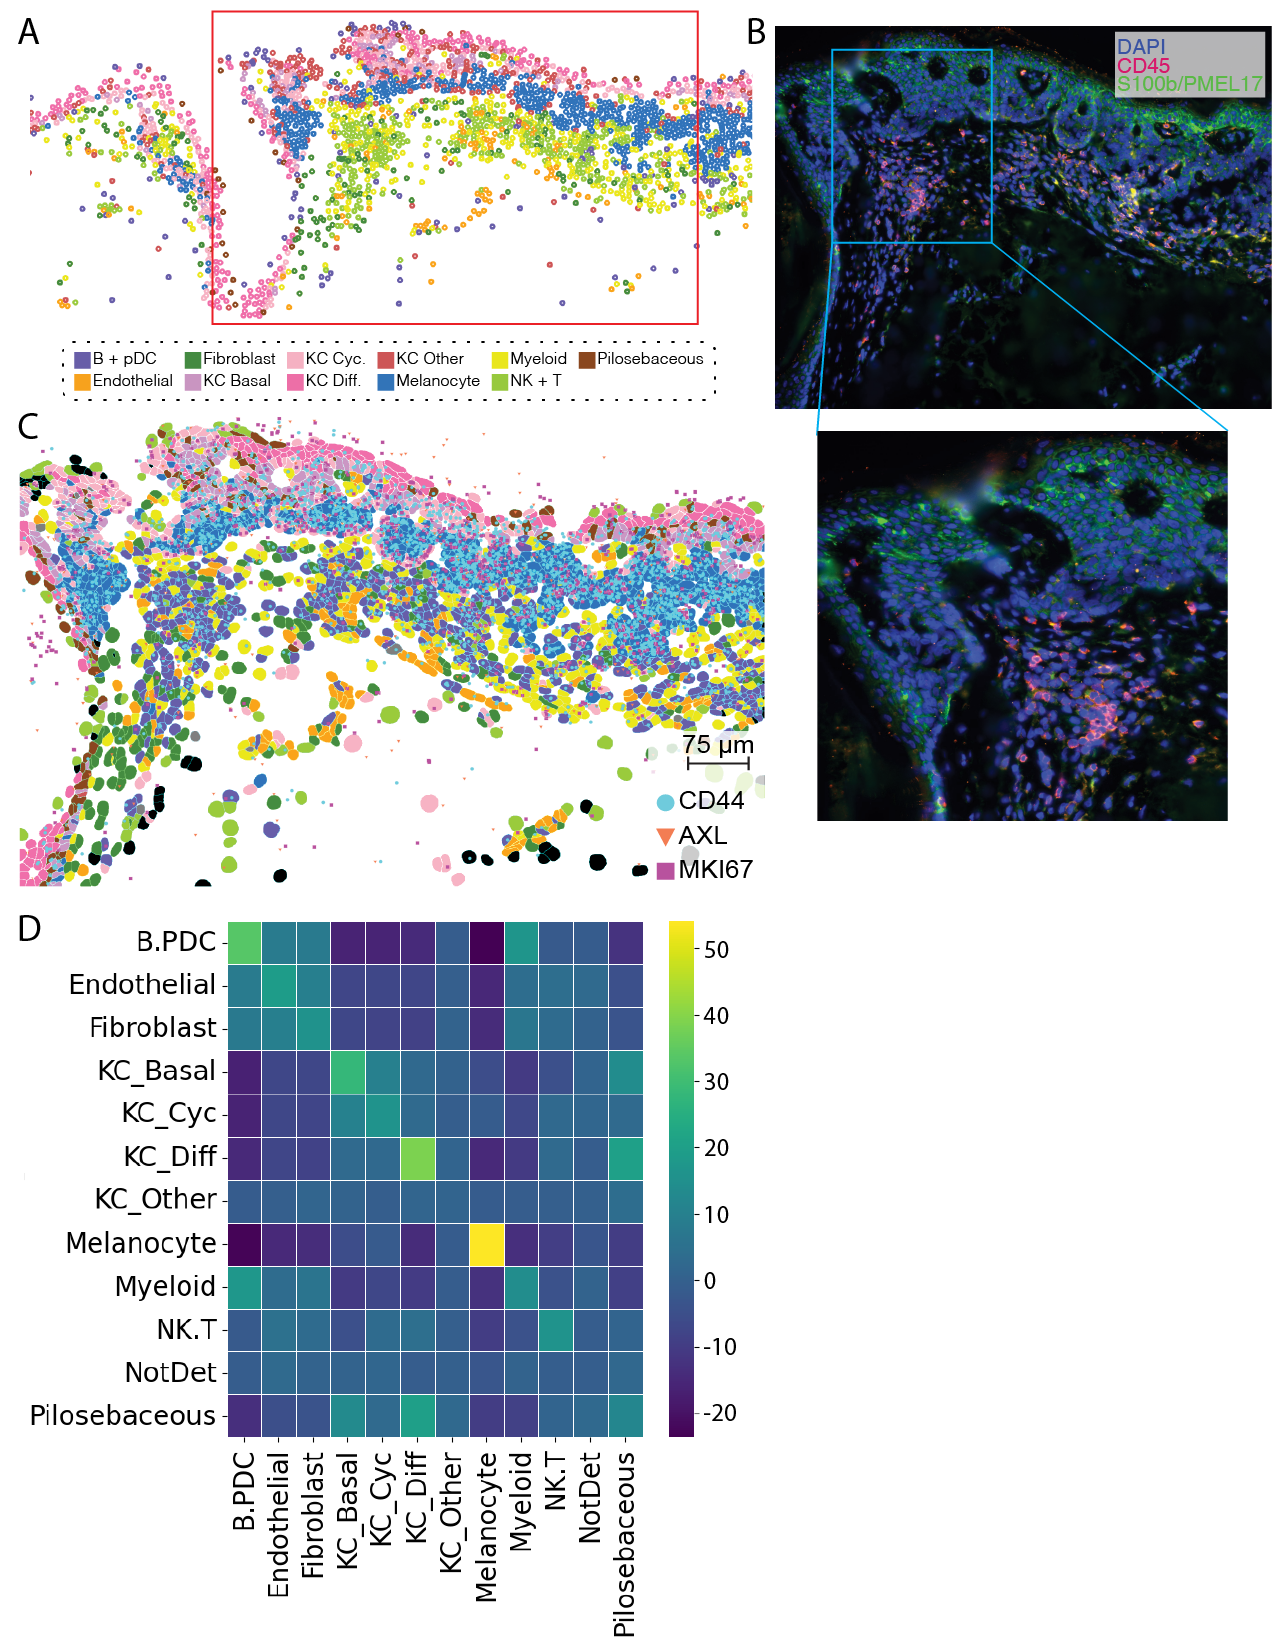
\includegraphics[width=0.85\columnwidth]{Chapter4/Figures/Chapter4_Fig3_CosMx_transcript_colocalisation2.png}
    \caption[Spatial analysis of cells colocalisation in a melanoma tissue]{Spatial analysis of cells colocalisation in a melanoma tissue. (A) The cell type annotation clearly shows the melanocyte layer blue at the bottom layer of the epidermis. (B) The immunostaining of the adjacent tissue is shown in A for DAPI, CD45 and PMEL markers. The zoom-in image of the region with high expression of PMEL marker. (C) The cell segmentation overlayed by single transcript expression of melanoma-associated gene markers KMI67, CD44, and AXL co-localise to melanoma tissue. (D) The neighbourhood enrichment analysis of the same FOV showed the enrichment of interaction among Melanocyte cells }
    \label{Chap4:CosMX_transcript_colo}
    
\end{figure}

\subsection{Variation in the tumour microenvironment as a potential predictive model in colorectal cancer with IMC data}
\subsubsection{Quantitative correlation of spatial heterogeneity and clinical prognosis}
Given the availability of MSI status, treatment and outcome data for the patients in the IMC dataset (Table \ref{table:Chapt4_IMC_patient_metadata}), we aimed to assess whether the cell neighbourhoods were associated with clinical outcomes or genetic alterations in CRC. First, we established the Delaunay network across the ROIs to generate the sparse network representation of the cell neighbourhood. For each individual patient, we assessed the spatial heterogeneity of each ROI and visualised the heterogeneity score. The boxplot in Fig \ref{Chap4:fig2:IMC_network_analysis}A shows the variation of the heterogeneity score across $42$ patients (out of $52$ patients with complete information Table \ref{table:Chapt4_IMC_patient_metadata}). A preliminary qualitative comparison between the patient with the lowest overall heterogeneity (CR079) and the one with the highest heterogeneity (CR101) suggested a correlation between the spatial neighbourhood and survival (Fig \ref{Chap4:fig2:IMC_network_analysis}B, C). Particularly, patient CR079 survived more than 3 years after being diagnosed, while CR101 lived less than a year (Table \ref{table:Chapt4_IMC_patient_metadata}). 

Next, we conducted quantitative testing of the significant correlation between the heterogeneity, MSI status and survival using the non-parametric Mann-Whitney test. No significant differences were observed in the correlation between heterogeneity and MSI status $pval=0.05$ (Fig \ref{Chap4:fig2:IMC_network_analysis}D). However, we found a strong correlation between lower spatial heterogeneity and long survival $pval=0.03$ ($>5 years mark$) (Fig \ref{table:Chapt4_IMC_patient_metadata}E). The finding of the correlation between cell heterogeneity agreed with some previous studies of CRC using spatial proteomic (\cite{schurch2020coordinated, li2017reference}). 

\begin{figure}
    \centering
    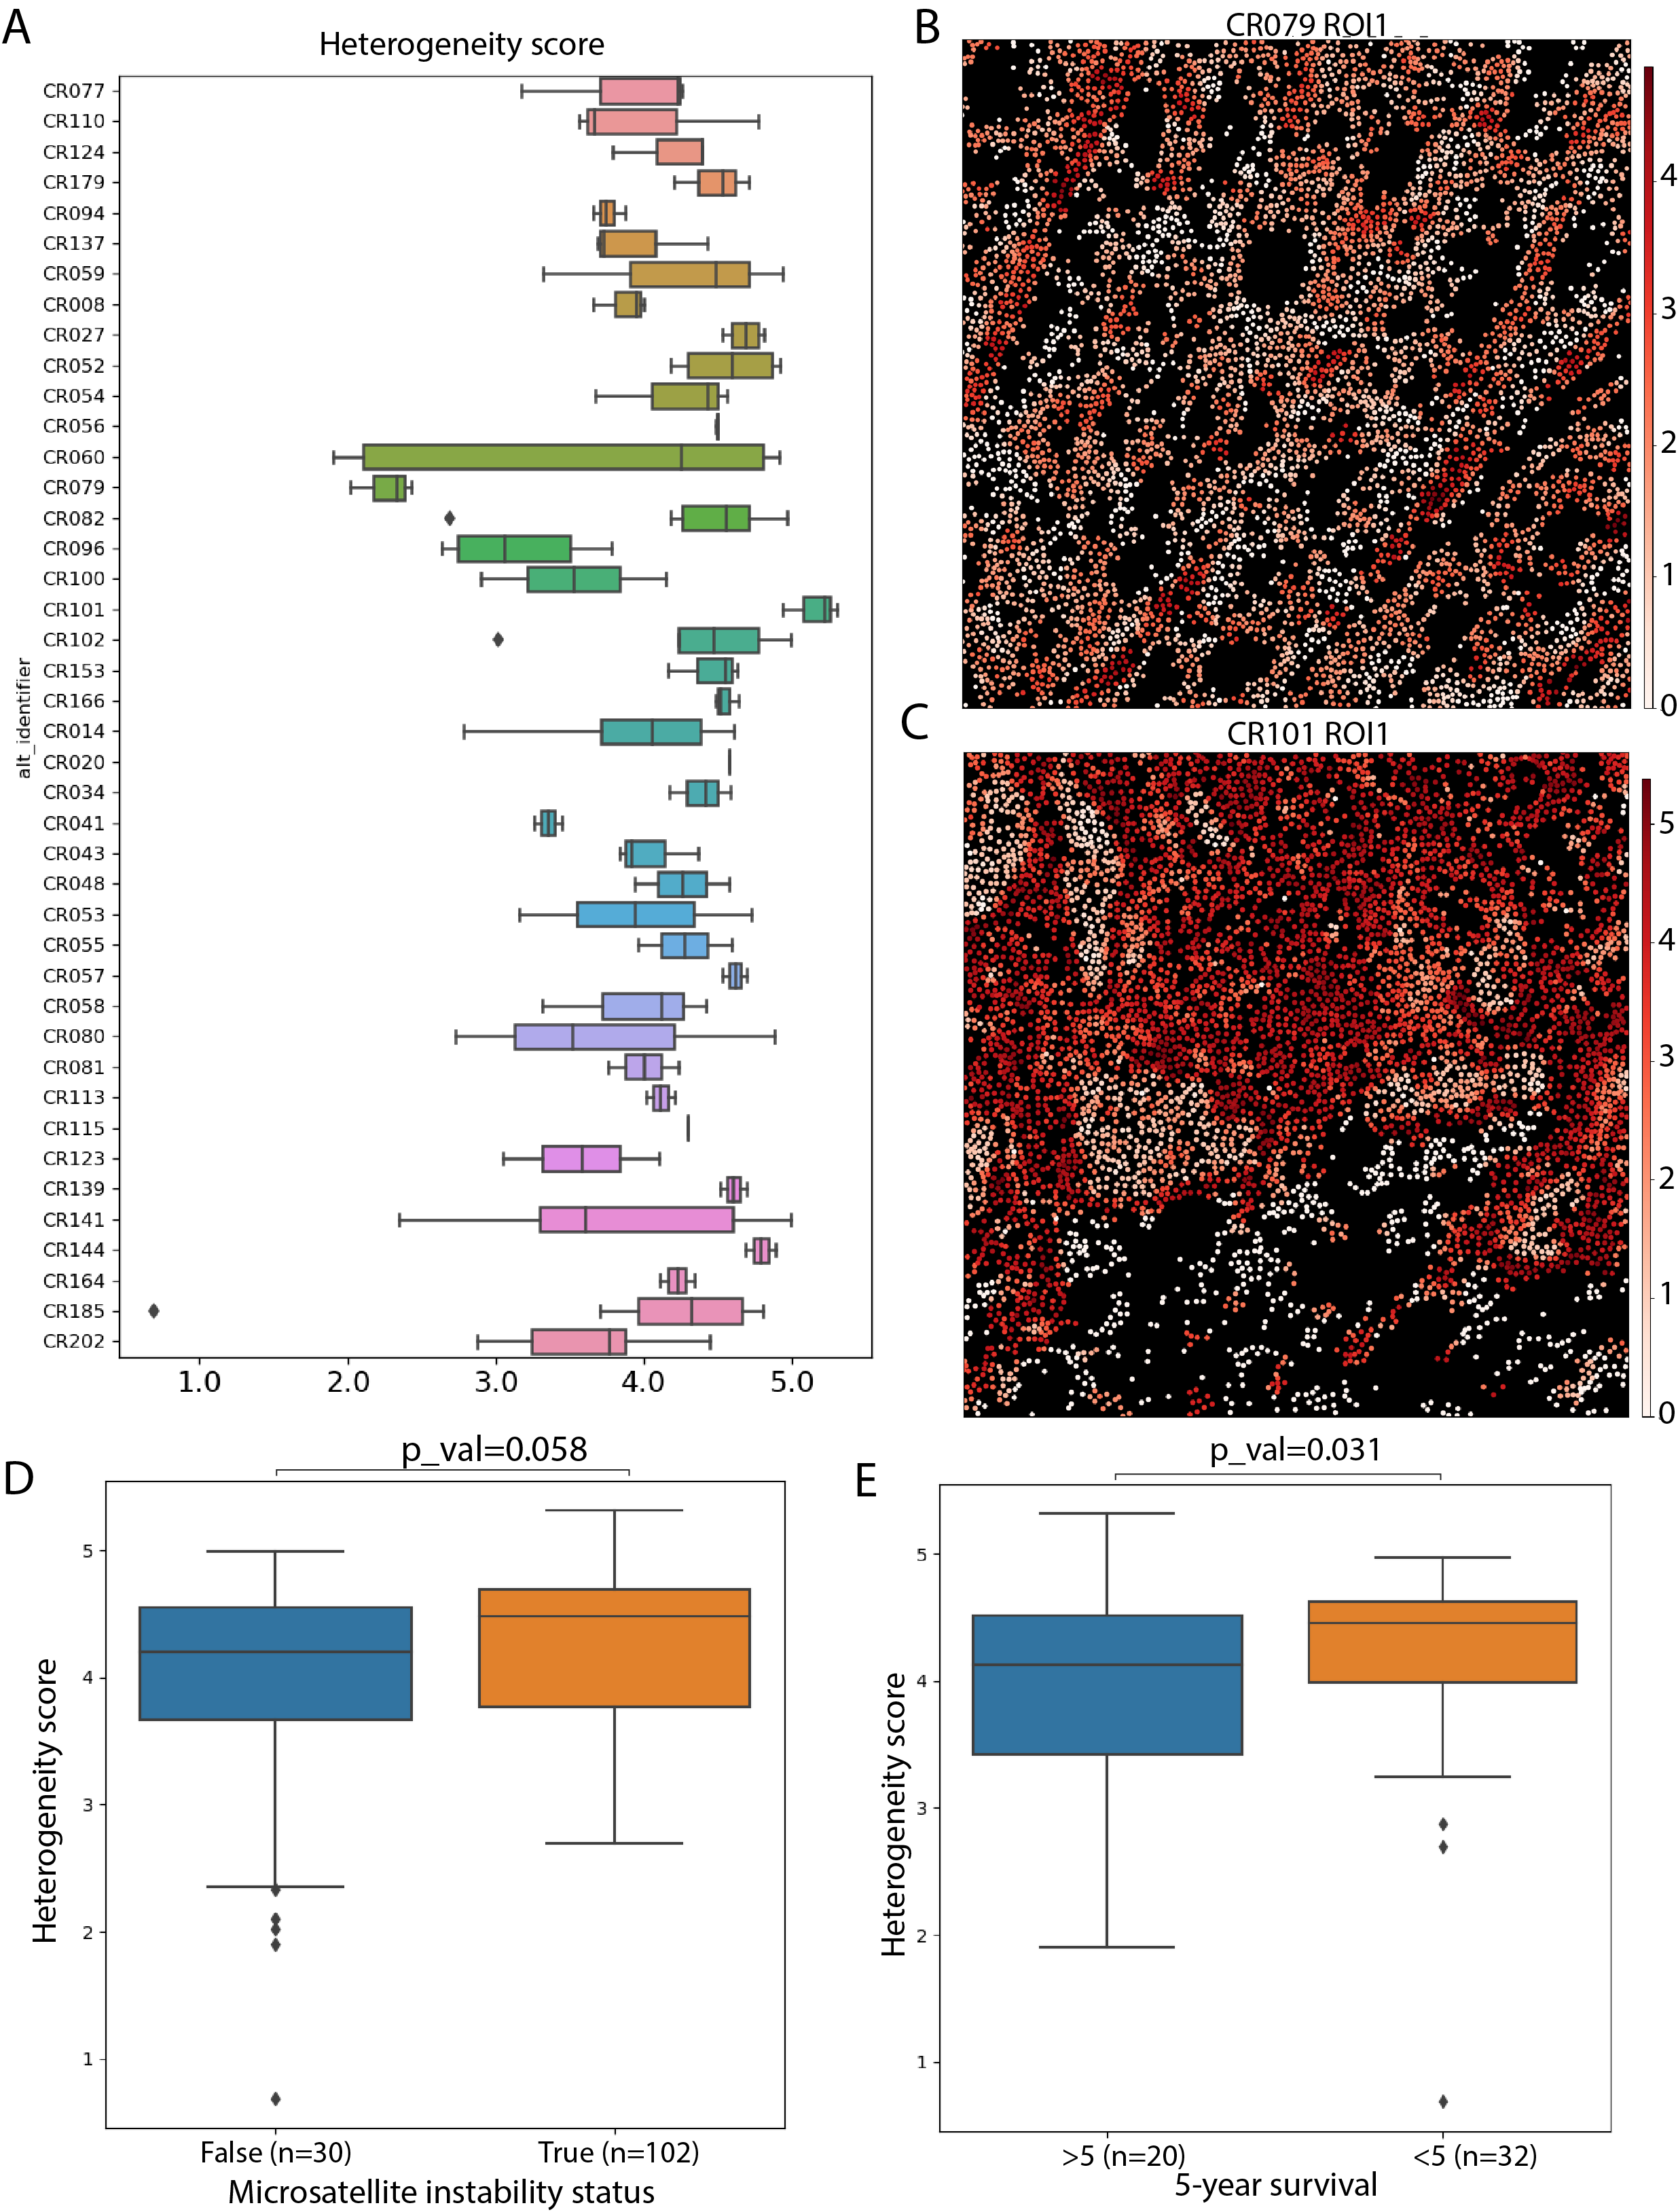
\includegraphics[width=0.9\columnwidth]{Chapter4/Figures/Chap4_figure6_IMC_network_analysis.png}
    \caption[IMC spatial cellular neighbourhood network analysis across the dataset]{The spatial cellular neighbourhood network analysis across all patients. (A) Boxplot shows the variation of cellular heterogeneity analysis in $42$ patients with the MSI information available from the IMC dataset. (B) An ROI from the patient CR079 with the lowest heterogeneity. (C) The patient CR101 displayed the highest overall heterogeneity. (D) signification test of cell network analysis against MSI status and survival information across samples}
    
    \label{Chap4:fig2:IMC_network_analysis}
    
\end{figure}
\subsubsection{Multi-sample spatial neighbourhood enrichment and the correlation between cell type distance and CRC prognosis}
The results presented so far mainly focused on the prediction ability of the MOSAP heterogeneity analysis. However, it is also possible to derive the correlation between cell type neighbourhood and clinical outcome through neighbourhood enrichment analysis and pairwise distance. This analysis aimed to determine whether the frequency of cell type neighbourhood could be associated with clinical outcomes. More specifically, we performed neighbourhood enrichment analysis to identify the pair of cell types in the neighbourhood that were over-represented or over-depleted in the neighbourhood network across the ROIs. Given the $11$ cell types, a total of $55$ pairs were determined and measured. The cell type labels within each ROI were shuffled $1000$ times while maintaining the neighbourhood connectivity. As shown in Figure \ref{Chap4:fig_IMC_res2}A, we could identify the enrichment for the neighbourhood between $16$ pairs of cell types (top $16$ positive enrichment scores) and depletion neighbourhood of $12$ pairs (bottom $12$ negative enrichment scores). Overall, we observed that the immune cell subsets (\ie CD8 T-cell, CD4 T-cell, macrophages and B-cell) and stromal cells appeared to be neighbored more than the neighbourhood cancer-immune cells (\ie epithelial/tumour cells, P53+ tumour). From the neighbourhood enrichment analysis, we carried out the correlation between the enrichment score and MSI status as well as survival outcome (Fig \ref{Chap4:fig_IMC_res2}B). The neighbourhood enrichment score between the two pairs of P53+ tumour-stromal and P53+ tumour with itself was significantly different between the group of patients with MSI-MSS. Meanwhile, significant differences between long-short survival groups were mostly observed among the immune cells such as CD4 T-cell, CD8 T-cell and Macrophages (Fig \ref{Chap4:fig_IMC_res2}C). 

To further assess how the relative distribution of each cell type was associated with the prognosis, we extracted the pairwise distance between neighbouring cells in the MOSAP spatial radius network. The distance values were again grouped by the MSI status. Wilcoxon rank sum test was applied to differentiate the distance between MSI and MSS status. We observed significant changes in the MSI status with respect to the distance between the cancer cell group (including tumour, P53+ tumour and proliferative) and CD4 T-cell as well as B cells. The distances of stroma cell with CD4 T-cells was also remarkably different between the two MSI subgroups. This is also consistent with the previous result from neighbourhood enrichment analysis. Similarly, a significant test was performed to derive the relation between cell type distance and survival outcome. Consistently, we identified that the most significant between the long and short-survival patient groups was associated with the distance between immune cells such as B-cells, NK-cells and Macrophages.  

\begin{figure}
    \centering
    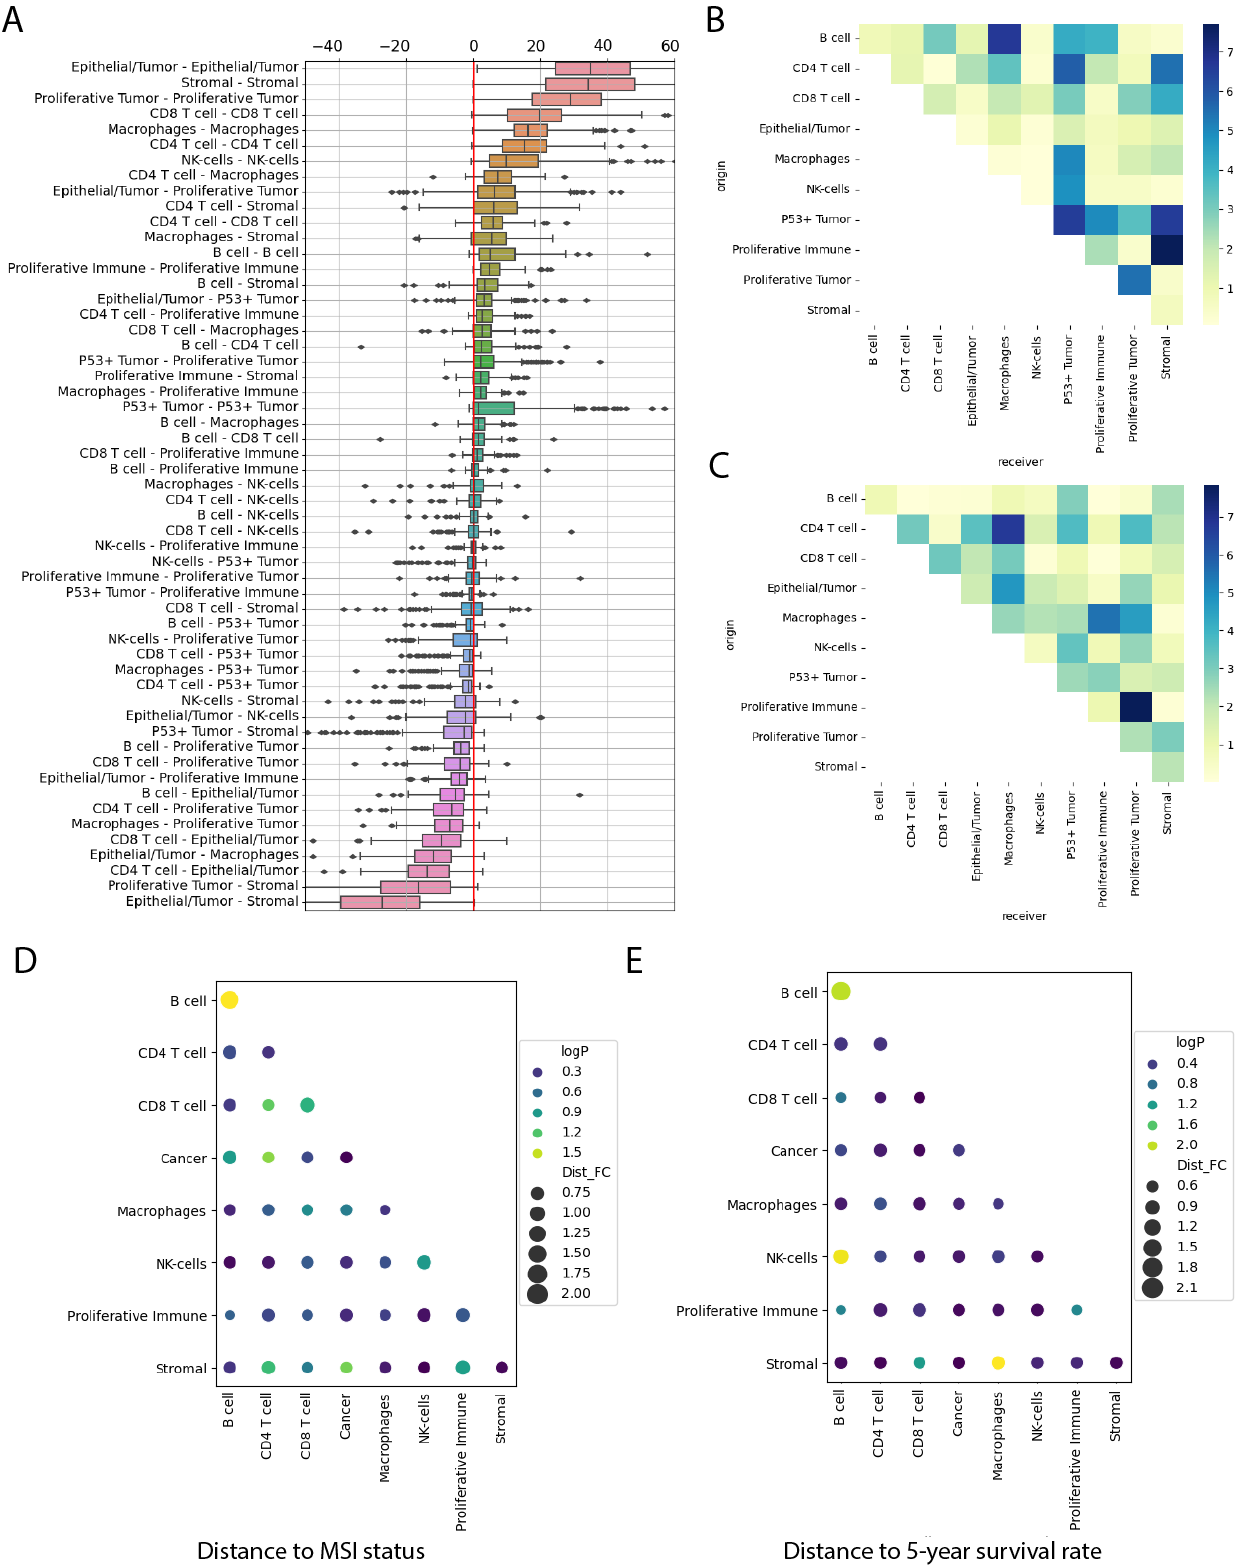
\includegraphics[width=\columnwidth]{Chapter4/Figures/Chapt4_figure4_IMC_sig_test.png}
    \caption[The association of cellular neighbourhood with the MSI status and clinical outcome]{The association of cellular neighbourhood with the MSI status and clinical outcome. (A) The box plot shows a variation of the neighbourhood enrichment scores between every pair of cell types across 172 ROIs. (B, C) Significant testing of the variation of cell types' neighbourhood enrichment scores against MSI status (B) and 5-year survival rate (C), respectively (scale bar indicates the $-log(pval)$). (D, E) The association of cell-cell neighbourhood distance and the MSI status (D) and 5-year survival rate)}
    \label{Chap4:fig_IMC_res2}
    
\end{figure} 

\section{Discussion}
In this chapter, we introduced the $Mosadata$ object, a sample-centric data type specifically designed to handle multi-sample and/or multimodal data processing. The $Mosadata$ object is integrated within the MOSAP platform, which provides various features for constructing cellular spatial networks and deriving quantitative measurements from the spatial-omic data. The robustness of the MOSAP platform was demonstrated through the quantitative analysis of two distinct types of spatial-omic data, namely CosMx for spatial transcriptomics in the skin cancer dataset and IMC for spatial proteomics in the CRC dataset. By utilising the MOSAP platform, we were able to gain valuable insights into the complex cellular composition and heterogeneity of the two datasets. 

Regarding the skin cancer dataset, the CosMx data was generated in conjunction with five other omics technologies (including scRNA-seq, RNAscope, Visium, GeoMx and multiplexed IHC), which collectively contributed to a comprehensive atlas of skin cancer manuscript. We thoroughly studied the cell-cell interaction through cell colocalisation and cell neighbourhood analyses. The MOSAP network analysis was applied to compare of intra-tumour heterogeneity and inter-tumour comparison across three skin cancer subtypes. We believe that the comparison of the complex cellular composition of TME heterogeneity and cellular interactions is crucial for understanding the distinct initiation and progression mechanisms of each skin cancer type \cite{stonesifer2021immune,wang2016crosstalk}. Additionally, it is important to acknowledge the contribution of other team members in providing valuable reference cell types for the CosMx dataset from single-cell RNA analysis and other complementary spatial data. The $11$ cell types of CosMx data were annotated by transferring cell labels from sc-RNAseq, which is the result of the collaborative efforts between other co-authors in the project, particularly Xinnan Jin and Laura Grice.        

While several recent studies have extensively characterised tumour-immune cell type, the investigation of how spatial organization and the association of cell neighbourhood across TME in CRC can affect the clinical outcome is still limited (\cite{schurch2020coordinated, kather2017silico,newell2018high,blise2022single}). Through the analysis of spatial cellular network and neighbourhood enrichment analysis, we were able to capture the high-level spatial pattern (\ie inter-tumour heterogeneity, neighbourhood enrichment) of the TMEs and the spatial architectures associated with clinical outcome. Our heterogeneity analysis results were in concordance with the findings of several other studies in relation to CRC survival (\cite{schurch2020coordinated, li2017reference}). While we observed no significant connection between spatial heterogeneity and MSI status, the neighbourhood enrichment analyses suggested that the enrichment of neighbourhoods between P53+ tumour cells and CD4 T-cells, stromal cells, and B cells were highly correlated to the MSI positive. A similar observation was identified by the pairwise distance between cancer cells (grouped of Proliferative and P53+ tumour cells) and immune cells (most significant with CD4 T-cell and B cells) \ref{Chap4:fig_IMC_res2}. Given the information that we have for the CRC dataset, there are some limitations that exist with the annotation of MSI status and survival analysis. Clinically, the MSI screening classified a cancer tumour into low or high instability by testing the mismatch repair status of a segment of the DNA. For analysis purposes, the MSI status of our CRC dataset was binarised as True or False, which could over-generalise diagnostic interpretation.      

In summary, the successful application of the MOSAP platform highlights its potential as a powerful tool for analysing and interpreting spatial-omic data in various biological contexts. Through the application of MOSAP, we were able to conduct a comprehensive analysis of cellular neighbourhood networks and cell type heterogeneity in skin cancer and CRC cancer datasets. The implementation of $Mosadata$ also enabled the integration with the analysis of other spatial analysis frameworks (\ie squidpy \cite{palla2022squidpy}). As the availability of single-cell multi-omics data continues to increase, we hope that the spatial analysis feature of MOSAP can significantly accelerate the studies of cell-state variation in cancer and other diseases.   

\section{Appendix}
% Central Nervous System (CNS) 
\begin{sidewaystable}
  \centering
  \caption{IMC colorectal cancer metadata }
  \begin{longtable}{|c|c|c|c|c|c|c|c|c|}
\hline
 & \textbf{alt\_identifier} & \textbf{CHR\_17P\_DEL} & \textbf{MSI\_any} & \textbf{Reccurrance} & \textbf{Site} & \textbf{First\_metastatic\_site} & \textbf{DaysSurvival} & \textbf{5YearSurvival} \\
\hline
1 & CR041 & YES & false & recur & descending colon & liver & 989 & $<5$ \\
\hline
2 &CR043 & YES & false & recur & descending colon & liver & 1001 & $<5$ \\
\hline
3 & CR053 & YES & false & recur & ascending colon & lung & 882 & $<5$ \\
\hline
4 & CR055 & YES & false & unk & ascending colon & no data available & 2173 & $>5$ \\
\hline
5 & CR057 & YES & false & recur & cecum & liver & 685 & $<5$ \\
\hline
6 & CR060 & YES & false & recur & sigmoid colon & omentum & 831 & $<5$ \\
\hline
7 &CR077 & YES & false & recur & cecum & lung & 903 & $<5$ \\
\hline
8 & CR079 & YES & false & recur & sigmoid colon & liver & 901 & $<5$ \\
\hline
9 & CR080 & YES & false & recur & ascending colon & carcinomatosis & 510 & $<5$ \\
\hline
10 & CR094 & YES & false & recur & cecum & lung & 353 & $<5$ \\
\hline
11 & CR100 & YES & false & recur & cecum & lung & 576 & $<5$ \\
\hline
12 & CR141 & YES & false & recur & sigmoid colon & liver & 437 & $<5$ \\
\hline
13 & CR164 & YES & false & no recur & cecum & no data available & 3652 & $>5$ \\
\hline
14 & CR179 & YES & false & recur & sigmoid colon & retroperitoneum & 2188 & $>5$ \\
\hline
15 & CR020 & YES & false & recur & ascending & liver & 429 & $<5$ \\
\hline
16 & CR001 &  &  & recur & transverse  & lung & 1777 & $<5$ \\
\hline
17 & CR023 &  &  & recur & sigmoid & lung & 1981 & $>5$ \\
\hline
18 & CR038 &  &  & no recur & ascending colon &  & 2482 & $>5$ \\
\hline
19 & CR051 &  &  & recur & ascending colon & abd wall & 272 & $<5$ \\
\hline
20 & CR052 &  & false & recur & cecum & liver & 747 & $<5$ \\
\hline
21 & CR059 &  & true & recur & cecum & lung & 485 & $<5$ \\
\hline
22 & CR067 & & & no recur & descending colon &  & 2681 & $>5$ \\
\hline
23 & CR084 & & & recur & ascending colon & pelvic masses & 633 & $<5$ \\

\hline
24 & CR097 & & & no recur & cecum &  & 3038 & $>5$ \\
\hline
25 & CR109 & & & recur & ascending colon & liver & 438 & $<5$ \\
\hline
26 & CR112 & & & recur & sigmoid colon & local/regional & 1986 & $>5$ \\
\hline
\multicolumn{4}{c}{\textit{Continued on the next page}} \\
% \hline
  \end{longtable}
  \label{table:Chapt4_IMC_patient_metadata}
\end{sidewaystable}

\begin{sidewaystable}
  \centering
  % % \caption{IMC colorectal cancer metadata (continue)}
  \begin{longtable}{|c|c|c|c|c|c|c|c|c|}
\hline
 & \textbf{alt\_identifier} & \textbf{CHR\_17P\_DEL} & \textbf{MSI\_any} & \textbf{Reccurrance} & \textbf{Site} & \textbf{First\_metastatic\_site} & \textbf{DaysSurvival} & \textbf{5YearSurvival} \\
\hline
27 & CR118 &  &  & recur & ascending colon & bone & 1012 &  $<5$ \\
\hline
28 & CR034 & NO & false & recur & ascending colon & liver & 405 & $<5$ \\
\hline
29 & CR054 & NO & false & recur & descending colon & abd wall & 1829 & $>5$ \\
\hline
30 & CR056 & NO & true & recur & cecum & cutaneous back tissue & 179 & $<5$ \\
\hline
31 & CR058 & NO & false & recur & sigmoid colon & no data available & 907 & $<5$ \\
\hline
32 & CR081 & NO & false & recur & cecum & bone & 946 & $<5$ \\
\hline
33 & CR082 & NO & true & no recur & transverse &   & 2176 & $>5$ \\
\hline
34 & CR096 & NO & false & recur & splenic flexure & carcinomatosis & 749 & $<5$ \\
\hline
35 & CR101 & NO & true & recur & transverse & CNS & 357 & $<5$ \\
\hline
36 & CR102 & NO & false & recur & ascending colon & liver & 906 & $<5$ \\
\hline
37 & CR110 & NO & true & no further update & transverse & no data available & 2009 & $>5$ \\
\hline
38 & CR113 & NO & false & recur & cecum & lung & 3627 & $>5$ \\
\hline
39 & CR137 & NO & false & recur & sigmoid colon & liver & 513 & $<5$ \\
\hline
40 & CR139 & NO & false & no recur & ascending colon &   & 2272 & $>5$ \\
\hline
41 & CR144 & NO & true & recur & ascending colon & carcinomatosis & 453 & $<5$ \\
\hline
42 & CR153 & NO & false & no recur & cecum &   & 1993 & $>5$ \\
\hline
43 & CR166 & NO & false & recur & descending colon & liver & 1917 & $>5$ \\
\hline
44 &CR008 & NO & false & recur & sigmoid & bone & 1793 & $<5$ \\
\hline
45 & CR014 & NO & true & recur & transverse & retroperitoneal & 817 & $<5$ \\
\hline
46 &CR027 & NO & false & no further update  & cecum & no data available & 2137 & $>5$ \\
\hline
47 & CR048 & NO & true & no recur & transverse &   & 1916 & $>5$ \\
\hline
48 & CR115 & NO & false & recur & appendix & local/regional & 1045 & $<5$ \\
\hline
49 & CR123 & NO & false & no recur & sigmoid & no data available & 468 & $<5$ \\
\hline
50 & CR124 & NO & false & no recur & sigmoid &   & 2757 & $>5$ \\
\hline
51 & CR185 & NO & false & recur & descending colon & lung & 2395 & $>5$ \\
\hline
52 & CR202 & NO & true & no recur & transverse & no data available & 2017 & $>5$ \\
\hline
  \end{longtable}
\end{sidewaystable}

% \label{Sec:4.3_quantitative_validation}	%CREATE YOUR OWN LABEL.
% \subsection{}
% ********* Enter your text below this line: ********

% ***************************************************
% \bibliographystyle{elsarticle-num}

% \bibliography{./References/Bibliography}